% ── Desarrollo ───────────────────────────────────────────────────────────────
\section{Desarrollo}

\subsection{Descripción General del Sistema}
El sistema, denominado Portal Digital TUPA - UNSAAC, está compuesto por tres
capas: una aplicación cliente construida en React que consume una API REST
desarrollada en Node.js/Express, la cual a su vez persiste la información en
una base de datos relacional PostgreSQL. El sistema contempla dos tipos de
usuario con necesidades y permisos distintos.

\subsubsection{Usuarios y Roles}
El \emph{payload} del token JWT distingue únicamente dos roles,
\texttt{USER} y \texttt{ADMIN}, que son los que gobiernan el control de acceso
de la API. El campo \texttt{rol\_admin} de la tabla \texttt{usuario\_admin}
(\texttt{ADMIN} o \texttt{SUPER\_ADMIN}) se transporta en el token como
\texttt{subRole} pero, en la versión entregada, no diferencia permisos.

\begin{itemize}
    \item \textbf{Estudiante} --- rol \texttt{USER}, tabla
    \texttt{usuario\_general}: puede consultar el catálogo público de
    trámites, iniciar una solicitud mediante un asistente guiado de seis
    pasos, cargar los documentos requeridos, registrar su comprobante de
    pago, dar seguimiento a sus expedientes y recibir notificaciones sobre el
    estado de estos.
    \item \textbf{Administrador} --- rol \texttt{ADMIN}, tabla
    \texttt{usuario\_admin}: puede revisar la cola de solicitudes pendientes,
    validar o rechazar los documentos cargados, registrar observaciones y
    decisiones sobre cada expediente, y gestionar el catálogo de trámites y
    los usuarios del sistema.
\end{itemize}

\subsection{Requerimientos}

\subsubsection{Requerimientos Funcionales}
\apatable{%
\begin{tabular}{@{}p{1.3cm}>{\raggedright\arraybackslash}p{10.6cm}p{2.6cm}@{}}
\toprule
\textbf{Código} & \textbf{Descripción} & \textbf{Estado} \\
\midrule
RF-01 & Consulta pública del catálogo de trámites, con filtros por búsqueda, categoría, costo y plazos. & Implementado \\
RF-02 & Inicio de sesión de estudiantes y administradores mediante credenciales del sistema. & Implementado \\
RF-03 & Registro de cuenta con correo institucional y activación por enlace enviado por correo. & Implementado \\
RF-04 & Recuperación de contraseña mediante código de seis dígitos enviado por correo. & Implementado \\
RF-05 & Creación de una solicitud en borrador y avance del asistente por los pasos 1 a 6. & Implementado \\
RF-06 & Carga de comprobante de pago y documentos requeridos por requisito. & Implementado \\
RF-07 & Generación automática de número de expediente al confirmar el envío. & Implementado \\
RF-08 & Rastreo público por número de expediente, con datos del solicitante anonimizados. & Implementado \\
RF-09 & Notificaciones de estado y observaciones para el usuario. & Implementado \\
RF-10 & Cola administrativa de solicitudes pendientes con revisión por expediente. & Implementado \\
RF-11 & Decisión administrativa sobre validación de documentos y estado de la solicitud. & Implementado \\
RF-12 & Gestión del catálogo y activación/desactivación de usuarios y trámites. & Implementado \\
RF-13 & Integración con pasarela de pagos y autenticación con Google. & No implementado \\
\bottomrule
\end{tabular}%
}{Requerimientos funcionales del sistema y su estado de implementación.}{tab:rf}

La tabla anterior se valida directamente con las rutas expuestas por el backend
(\texttt{/api/auth}, \texttt{/api/procedures}, \texttt{/api/requests},
\texttt{/api/admin}) y con los componentes de navegación definidos en
\texttt{frontend/src/App.jsx}. El requerimiento RF-13 queda fuera del alcance
de la versión entregada: el endpoint \texttt{POST /api/auth/google} responde
\texttt{501 Not Implemented} de forma explícita, y el pago se registra
mediante la carga manual de un comprobante en lugar de una pasarela.

\subsubsection{Requerimientos No Funcionales}
\apatable{%
\begin{tabular}{@{}p{1.4cm}>{\raggedright\arraybackslash}p{13.2cm}@{}}
\toprule
\textbf{Código} & \textbf{Descripción} \\
\midrule
RNF-01 & Las contraseñas de los usuarios deben almacenarse cifradas mediante una función de hash (\texttt{bcrypt}, 10 rondas de sal), nunca en texto plano. \\
RNF-02 & El acceso a los recursos protegidos de la API debe requerir un token JWT válido en la cabecera \texttt{Authorization}. \\
RNF-03 & Las rutas bajo \texttt{/api/admin} deben restringirse a portadores de un token con rol \texttt{ADMIN}. \\
RNF-04 & Todas las consultas a la base de datos deben usar sentencias parametrizadas para prevenir inyección SQL. \\
RNF-05 & Los endpoints sensibles de autenticación deben limitar la cantidad de intentos por dirección IP dentro de una ventana de tiempo. \\
RNF-06 & Los archivos cargados deben restringirse por tipo (PDF, JPG, JPEG, PNG) y por tamaño máximo (5~MB). \\
RNF-07 & Los mensajes de error de autenticación no deben permitir deducir qué correos están registrados en el sistema. \\
RNF-08 & La interfaz debe ser consumible desde un navegador web moderno, comunicándose con el backend mediante peticiones HTTP habilitadas por CORS. \\
\bottomrule
\end{tabular}%
}{Requerimientos no funcionales del sistema.}{tab:rnf}

\subsection{Arquitectura del Sistema}

\subsubsection{Arquitectura General}
La Figura~\ref{fig:arquitectura} presenta la arquitectura general del
sistema, organizada en tres capas desacopladas que se comunican mediante
peticiones HTTP/JSON.

\apafigure{%
\begin{tikzpicture}[node distance=1.6cm and 2.4cm]
    \node[bloque] (cliente) {Cliente Web\\(React + Vite)};
    \node[bloque, right=of cliente] (api) {API REST\\(Node.js + Express)};
    \node[bloque, right=of api] (bd) {Base de Datos\\(PostgreSQL)};

    \draw[flecha] (cliente) -- node[above, font=\footnotesize]{HTTP/JSON} (api);
    \draw[flecha] (api) -- node[above, font=\footnotesize]{SQL} (bd);
\end{tikzpicture}%
}{Arquitectura general del sistema en tres capas.}{fig:arquitectura}

\subsubsection{Arquitectura del Backend}
La organización real del backend en el repositorio es consistente con un
patrón Rutas--Controladores--Servicios, pero además incorpora utilidades y
miembros adicionales de infraestructura:

\begin{itemize}
    \item \texttt{routes/}: define los siete prefijos de la API
    (\texttt{/api/auth}, \texttt{/api/users}, \texttt{/api/procedures},
    \texttt{/api/requests}, \texttt{/api/documents},
    \texttt{/api/notifications} y \texttt{/api/admin}) y enlaza cada ruta
    con su controlador.
    \item \texttt{controllers/}: reciben la solicitud HTTP, delegan la
    lógica a los servicios y responden con JSON. Todos los manejadores se
    envuelven en \texttt{asyncHandler}, de modo que cualquier promesa
    rechazada llega al middleware de errores en lugar de quedar sin capturar.
    \item \texttt{services/}: contienen la lógica de negocio y las
    consultas parametrizadas sobre PostgreSQL, incluidas la creación de
    solicitudes, la generación del expediente, la validación documental y la
    gestión de usuarios y trámites. Las operaciones que tocan varias tablas
    (registro, envío de solicitud, decisión administrativa) se ejecutan
    dentro de una transacción con \texttt{BEGIN}/\texttt{COMMIT} y bloqueo
    \texttt{SELECT \ldots FOR UPDATE} sobre la fila afectada.
    \item \texttt{middleware/}: implementa la autenticación JWT
    (\texttt{auth.middleware}), la autorización por rol, el limitador de
    intentos por IP (\texttt{rateLimit.middleware}), la carga de archivos
    mediante \texttt{multer} (\texttt{upload.middleware}) y el manejador
    centralizado de errores (\texttt{error.middleware}), que traduce los
    códigos de restricción de PostgreSQL a códigos HTTP de cliente.
    \item \texttt{db/}: centraliza el \emph{pool} de conexiones a PostgreSQL.
    \item \texttt{utils/}: contiene la generación del número de expediente
    (\texttt{generateExpediente}), la firma y verificación de tokens JWT
    (\texttt{jwt.util}) y las validaciones de entrada compartidas
    (\texttt{validate}), que normalizan identificadores y paginación.
\end{itemize}

\subsubsection{Arquitectura del Frontend}
La organización real del frontend presenta una división funcional por tipo de
vista, pero con una estructura más detallada que la descrita de forma general:

\begin{itemize}
    \item \texttt{pages/public}: páginas de acceso público como landing,
    catálogo, búsqueda y rastreo de expedientes.
    \item \texttt{pages/auth}: flujo de autenticación (inicio de sesión,
    registro, activación de cuenta y recuperación de contraseña).
    \item \texttt{pages/student}: panel del estudiante, perfil, notificaciones,
    trámites propios y detalle de solicitudes.
    \item \texttt{pages/student/wizard}: asistente del flujo de solicitud
    en seis pasos.
    \item \texttt{pages/admin}: panel administrativo, cola de pendientes,
    validación documental, gestión de procedimientos, usuarios y reportes.
    \item \texttt{components/layout}: envolturas de página y el guardián de
    rutas \texttt{RequireAuth}, que redirige al inicio de sesión cuando no
    hay sesión activa y al panel correspondiente cuando el rol no coincide.
    \item \texttt{context/}: estado global de sesión (\texttt{AuthContext}) y
    del asistente de trámites (\texttt{WizardContext}), este último
    persistido en \texttt{localStorage} para que el avance no se pierda al
    recargar la página.
    \item \texttt{lib/api.js}: cliente HTTP único que adjunta el token de
    acceso, renueva automáticamente la sesión cuando expira y encola las
    peticiones que fallan mientras dura la renovación.
\end{itemize}

\subsection{Modelo de Base de Datos}

\subsubsection{Diagrama Entidad-Relación}
La Figura~\ref{fig:diagrama-entidad-relacion} presenta el diagrama
entidad-relación completo del modelo, generado a partir del esquema real de
PostgreSQL. Incluye las columnas \texttt{BYTEA} (\texttt{contenido},
\texttt{avatar\_contenido}) donde se almacena el contenido binario de
documentos y avatares directamente en la base de datos, en lugar de en el
disco del servidor.

\apafigure[p]{%
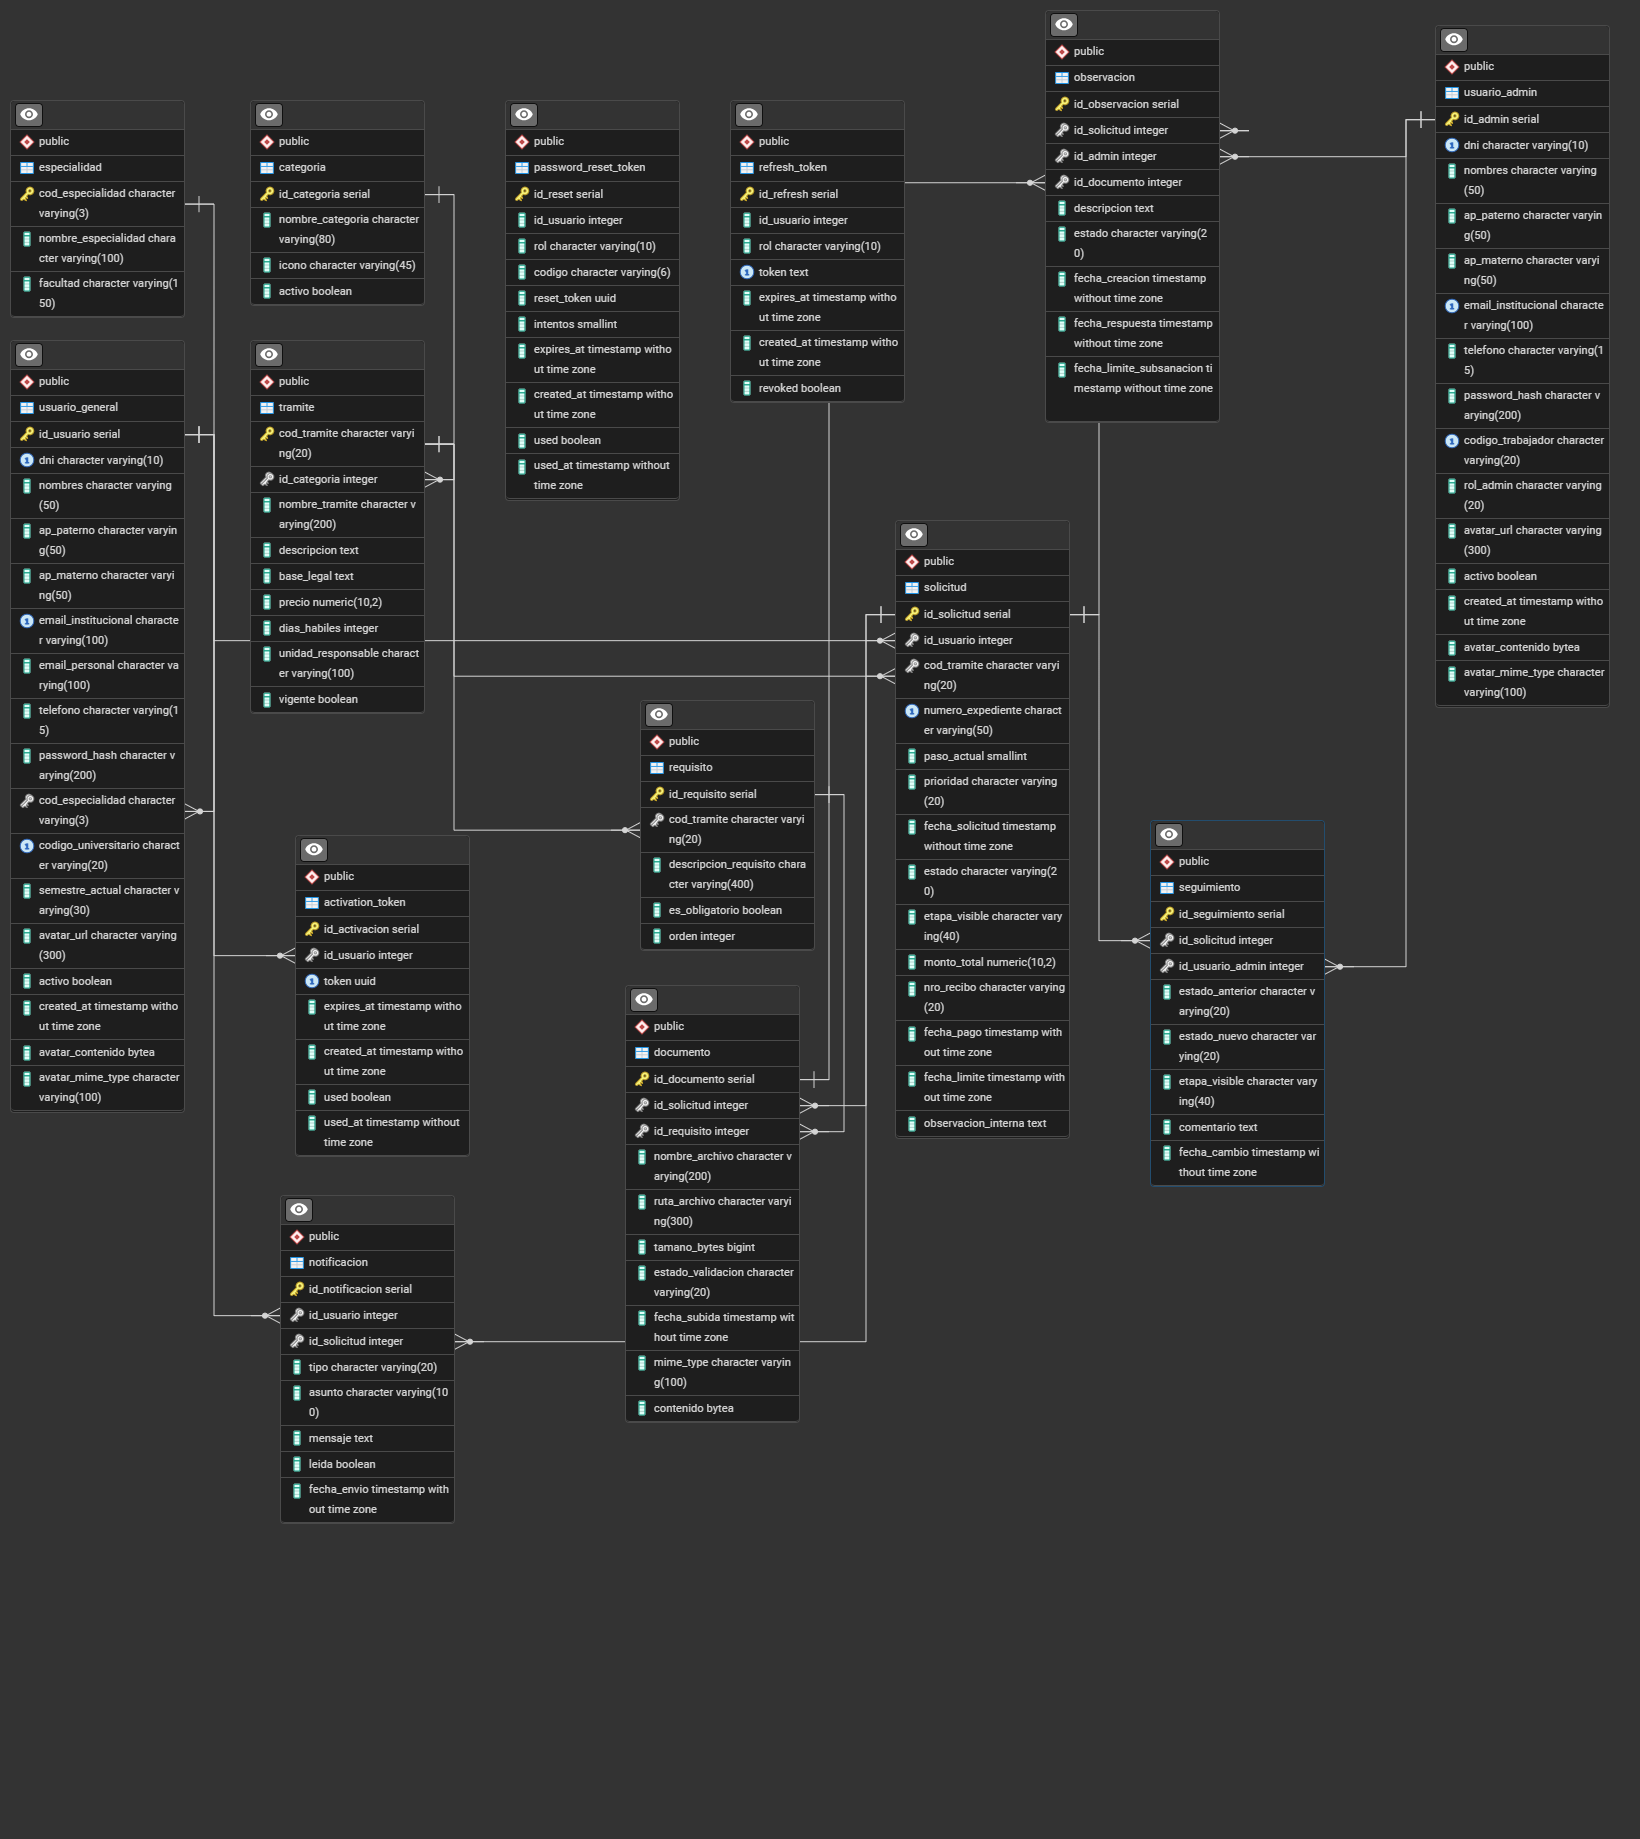
\includegraphics[width=\linewidth]{images/diagrama-entidad-relacion.png}%
}{Diagrama entidad-relación del modelo de base de datos de TUPA UNSAAC.}{fig:diagrama-entidad-relacion}

\subsubsection{Diccionario de Datos}
El modelo relacional está compuesto por catorce entidades: once del dominio
del negocio y tres dedicadas a la gestión de tokens de autenticación. La
Tabla~\ref{tab:diccionario} resume su propósito dentro del sistema.

\apatable{%
\begin{tabular}{@{}p{4.7cm}>{\raggedright\arraybackslash}p{10.0cm}@{}}
\toprule
\textbf{Entidad} & \textbf{Descripción} \\
\midrule
\texttt{especialidad} & Catálogo de especialidades/facultades a las que puede pertenecer un estudiante. \\
\texttt{usuario\_general} & Estudiantes que solicitan trámites; incluye datos institucionales, de contacto y el avatar almacenado como \texttt{BYTEA}. \\
\texttt{usuario\_admin} & Personal administrativo del sistema, con rol \texttt{ADMIN} o \texttt{SUPER\_ADMIN}. \\
\texttt{refresh\_token} & Tokens de renovación de sesión emitidos, con marca de revocación y vencimiento. \\
\texttt{activation\_token} & Enlaces de activación de cuenta, de un solo uso y con vigencia de 24 horas. \\
\texttt{password\_reset\_token} & Códigos de recuperación de contraseña, con contador de intentos y vigencia de 30 minutos. \\
\texttt{categoria} & Agrupación temática de los trámites del catálogo (p. ej. Certificados, Matrícula). \\
\texttt{tramite} & Catálogo oficial de procedimientos del TUPA: costo, plazo, base legal y vigencia. \\
\texttt{requisito} & Requisitos documentales obligatorios u opcionales asociados a cada trámite. \\
\texttt{solicitud} & Expediente creado por un estudiante para un trámite: estado, prioridad, número de expediente. \\
\texttt{documento} & Archivo digital cargado por el estudiante para cumplir un requisito específico; el contenido se guarda en la columna \texttt{contenido} de tipo \texttt{BYTEA}. \\
\texttt{observacion} & Observación registrada por un administrador sobre un documento o solicitud. \\
\texttt{seguimiento} & Bitácora histórica de cambios de estado de una solicitud. \\
\texttt{notificacion} & Alerta generada hacia un estudiante ante un evento relevante de su solicitud. \\
\bottomrule
\end{tabular}%
}{Diccionario de datos del modelo relacional.}{tab:diccionario}

\subsubsection{Relaciones Principales}
Un \texttt{usuario\_general} puede tener múltiples \texttt{solicitud} (una
por trámite iniciado); cada \texttt{solicitud} referencia un
\texttt{tramite} del catálogo. Cada \texttt{tramite} define uno o más
\texttt{requisito}, y cada \texttt{documento} cargado por el estudiante se
asocia opcionalmente a un \texttt{requisito} específico dentro de una
\texttt{solicitud}; los comprobantes de pago se registran como documentos sin
requisito asociado. Las tablas \texttt{observacion} y \texttt{seguimiento}
registran, respectivamente, las incidencias y el historial de cambios de
estado de una \texttt{solicitud}, ambas vinculadas al
\texttt{usuario\_admin} que las generó.

\subsubsection{Restricciones de Integridad}
El modelo aplica restricciones \texttt{CHECK} para limitar los valores
válidos de los campos de estado, evitando así estados inconsistentes a nivel
de base de datos:
\begin{itemize}
    \item \texttt{solicitud.estado} $\in$ \{\texttt{BORRADOR},
    \texttt{SOLICITADO}, \texttt{VERIFICANDO\_PAGO}, \texttt{PAGADO},
    \texttt{EN PROCESO}, \texttt{SUBSANACION}, \texttt{OBSERVADO},
    \texttt{COMPLETADO}, \texttt{ANULADO}, \texttt{RECHAZADO}\}.
    \item \texttt{solicitud.paso\_actual} restringido al intervalo $[1,6]$,
    de modo que el avance del asistente no puede salirse de rango.
    \item \texttt{documento.estado\_validacion} $\in$ \{\texttt{PENDIENTE},
    \texttt{APROBADO}, \texttt{RECHAZADO}\}.
    \item \texttt{observacion.estado} $\in$ \{\texttt{PENDIENTE},
    \texttt{SUBSANADO}, \texttt{CERRADO}\}.
    \item \texttt{refresh\_token.rol} y \texttt{password\_reset\_token.rol}
    $\in$ \{\texttt{USER}, \texttt{ADMIN}\}.
\end{itemize}
Adicionalmente, \texttt{solicitud.numero\_expediente} lleva una restricción
\texttt{UNIQUE}, y el esquema define índices sobre las columnas de búsqueda
frecuente (estado, fecha, expediente, usuario) y un índice parcial sobre las
notificaciones no leídas. El script de creación completo se encuentra en
\texttt{backend/sql/schema.sql}.

\subsection{Diseño de la API REST}
La API se organiza en siete módulos funcionales, cada uno bajo su propio
prefijo de ruta, que suman 38 endpoints. La Tabla~\ref{tab:api} resume los
módulos implementados y su conjunto de operaciones definido en la capa de
rutas del backend.

\apatable{%
\footnotesize
\begin{tabular}{@{}>{\raggedright\arraybackslash}p{2.3cm}>{\raggedright\arraybackslash}p{3.3cm}>{\raggedright\arraybackslash}p{9.2cm}@{}}
\toprule
\textbf{Módulo} & \textbf{Ruta} & \textbf{Endpoints implementados} \\
\midrule
Autenticación & \texttt{/api/auth} & \texttt{POST /login}, \texttt{POST /refresh}, \texttt{POST /logout}, \texttt{POST /register}, \texttt{POST /activate/:token}, \texttt{POST /resend-activation}, \texttt{POST /forgot-password}, \texttt{POST /resend-code}, \texttt{POST /verify-code}, \texttt{POST /reset-password}, \texttt{POST /google} (stub, responde \texttt{501}). \\
Perfil de usuario & \texttt{/api/users} & \texttt{GET /profile}, \texttt{PUT /profile}, \texttt{PUT /profile/password}, \texttt{POST /profile/avatar}, \texttt{GET /avatar/:role/:id}. \\
Catálogo de trámites & \texttt{/api/procedures} & \texttt{GET /}, \texttt{GET /categories}, \texttt{GET /:cod\_tramite}. \\
Solicitudes & \texttt{/api/requests} & \texttt{POST /}, \texttt{GET /}, \texttt{GET /:id}, \texttt{PATCH /:id/step}, \texttt{POST /:id/voucher}, \texttt{POST /:id/document/:id\_requisito}, \texttt{POST /:id/submit}, \texttt{GET /track/:numero\_expediente}. \\
Documentos & \texttt{/api/documents} & \texttt{GET /:id\_documento/view}, \texttt{DELETE /:id\_documento}. \\
Notificaciones & \texttt{/api/notifications} & \texttt{GET /}, \texttt{POST /read-all}, \texttt{PATCH /:id/read}. \\
Administración & \texttt{/api/admin} & \texttt{GET /stats}, \texttt{GET /requests}, \texttt{GET /requests/:id}, \texttt{POST /requests/:id/decision}, \texttt{POST /procedures}, \texttt{PATCH /procedures/:cod\_tramite/toggle}, \texttt{GET /users}, \texttt{PATCH /users/:id/toggle}. \\
\bottomrule
\end{tabular}%
}{Endpoints de la API REST del backend.}{tab:api}

Las rutas públicas son el catálogo completo (\texttt{/api/procedures}), el
rastreo por expediente (\texttt{GET /api/requests/track/:numero\_expediente}),
la descarga de avatares y todo el módulo de autenticación. El resto exige un
token válido, y las ocho rutas de \texttt{/api/admin} exigen además rol
\texttt{ADMIN}.

\subsubsection{Ciclo de Vida de una Solicitud}
El expediente avanza mediante un conjunto acotado de transiciones. Al crear
el borrador la solicitud nace en \texttt{BORRADOR}; la carga del comprobante
la mueve a \texttt{VERIFICANDO\_PAGO}; el envío
(\texttt{POST /api/requests/:id/submit}) verifica que todos los requisitos
obligatorios tengan documento adjunto, genera el número de expediente con
formato \texttt{EXP-AAAA-NNNNNN} y deja la solicitud en \texttt{SOLICITADO}.
A partir de ahí, la decisión administrativa
(\texttt{POST /api/admin/requests/:id/decision}) admite las acciones
\texttt{APROBAR}, \texttt{OBSERVAR}, \texttt{RECHAZAR} y \texttt{EN\_PROCESO}.
La acción \texttt{APROBAR} sólo cierra el expediente como \texttt{COMPLETADO}
si todos los requisitos obligatorios tienen su documento en estado
\texttt{APROBADO}; en caso contrario lo deja en \texttt{EN PROCESO}. Los
estados \texttt{COMPLETADO}, \texttt{RECHAZADO} y \texttt{ANULADO} son
terminales y no admiten nuevas decisiones. Cada transición inserta un registro
en \texttt{seguimiento} y genera una \texttt{notificacion} para el estudiante.

\subsection{Diseño de Interfaces}
El frontend implementado en React y Vite expone 33 rutas para los principales
escenarios del sistema. Las capturas que siguen fueron obtenidas navegando la
aplicación en ejecución mediante un navegador automatizado, con el backend
conectado a la base de datos del proyecto; por tanto, los datos que muestran
son los reales del sistema y no maquetas.

\subsubsection{Portal Público}
La navegación pública incluye la página de inicio, el catálogo de trámites,
el registro, la recuperación de contraseña y la consulta de expedientes, a
través de los componentes \texttt{LandingPage.jsx}, \texttt{Catalog.jsx},
\texttt{Registro.jsx}, \texttt{RecuperarPassword.jsx},
\texttt{TrackingSearch.jsx} y \texttt{TrackingResults.jsx}.

\apafigure{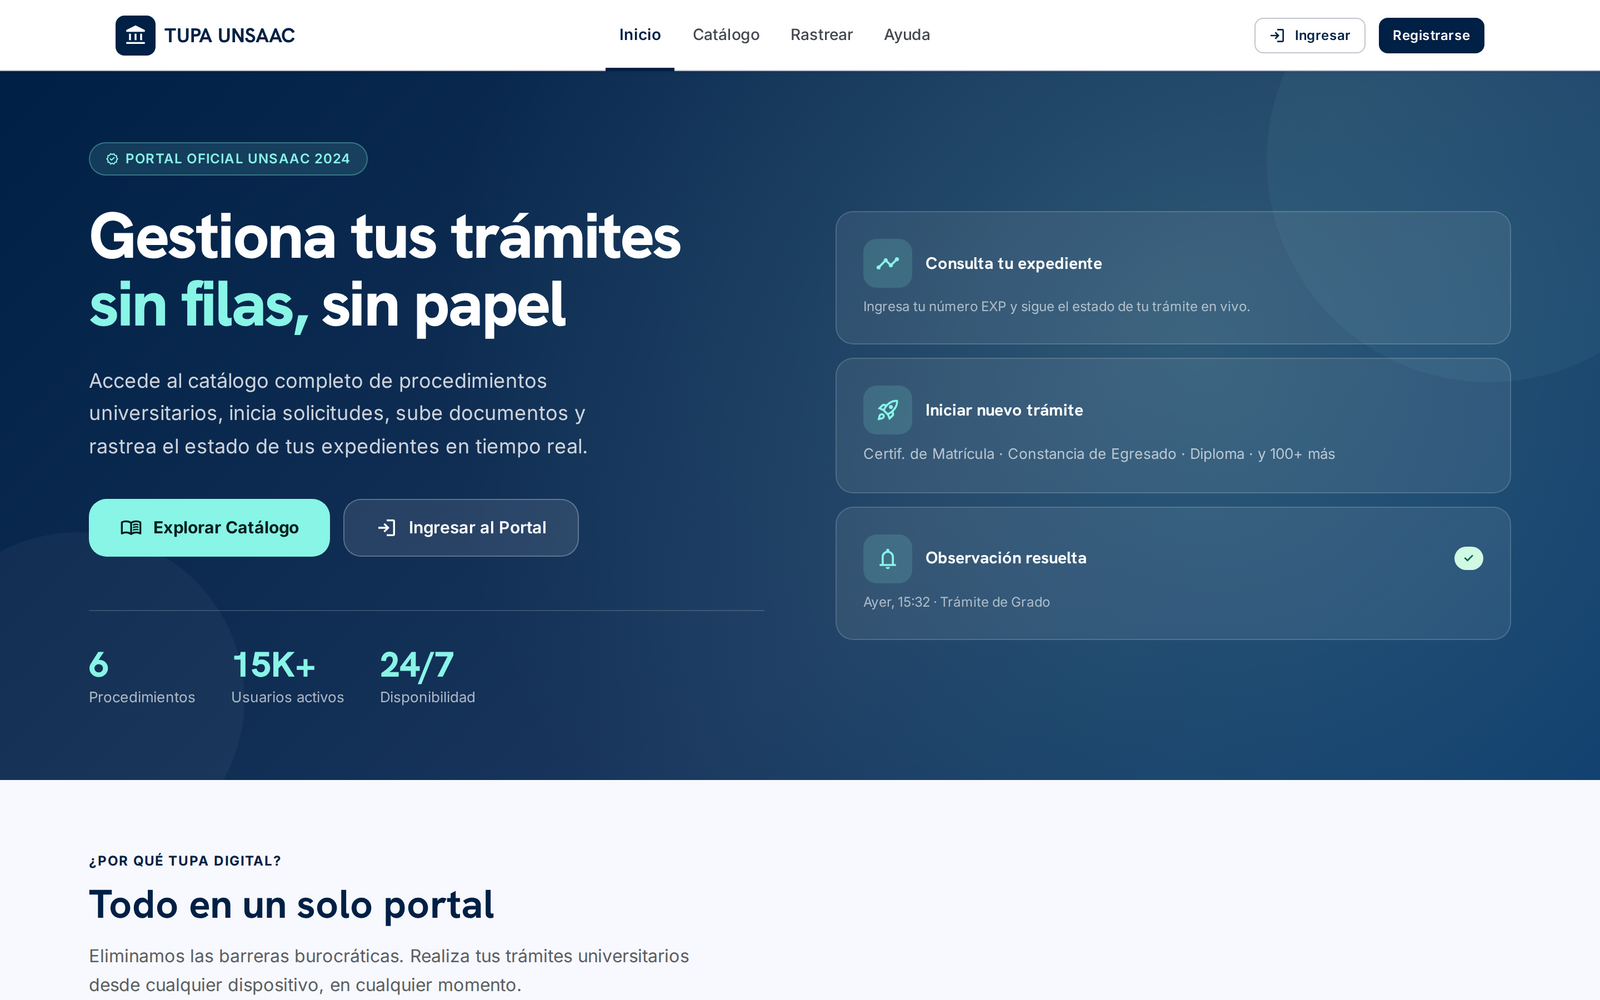
\includegraphics[width=0.95\textwidth]{images/capt-landing.png}}%
{Página de inicio del portal público (ruta \texttt{/}).}{fig:landing}

\apafigure{
\includegraphics[width=0.95\textwidth]{images/capt-login.png}}%
{Inicio de sesión con selector de tipo de usuario (ruta \texttt{/login}).}{fig:login}

\apafigure{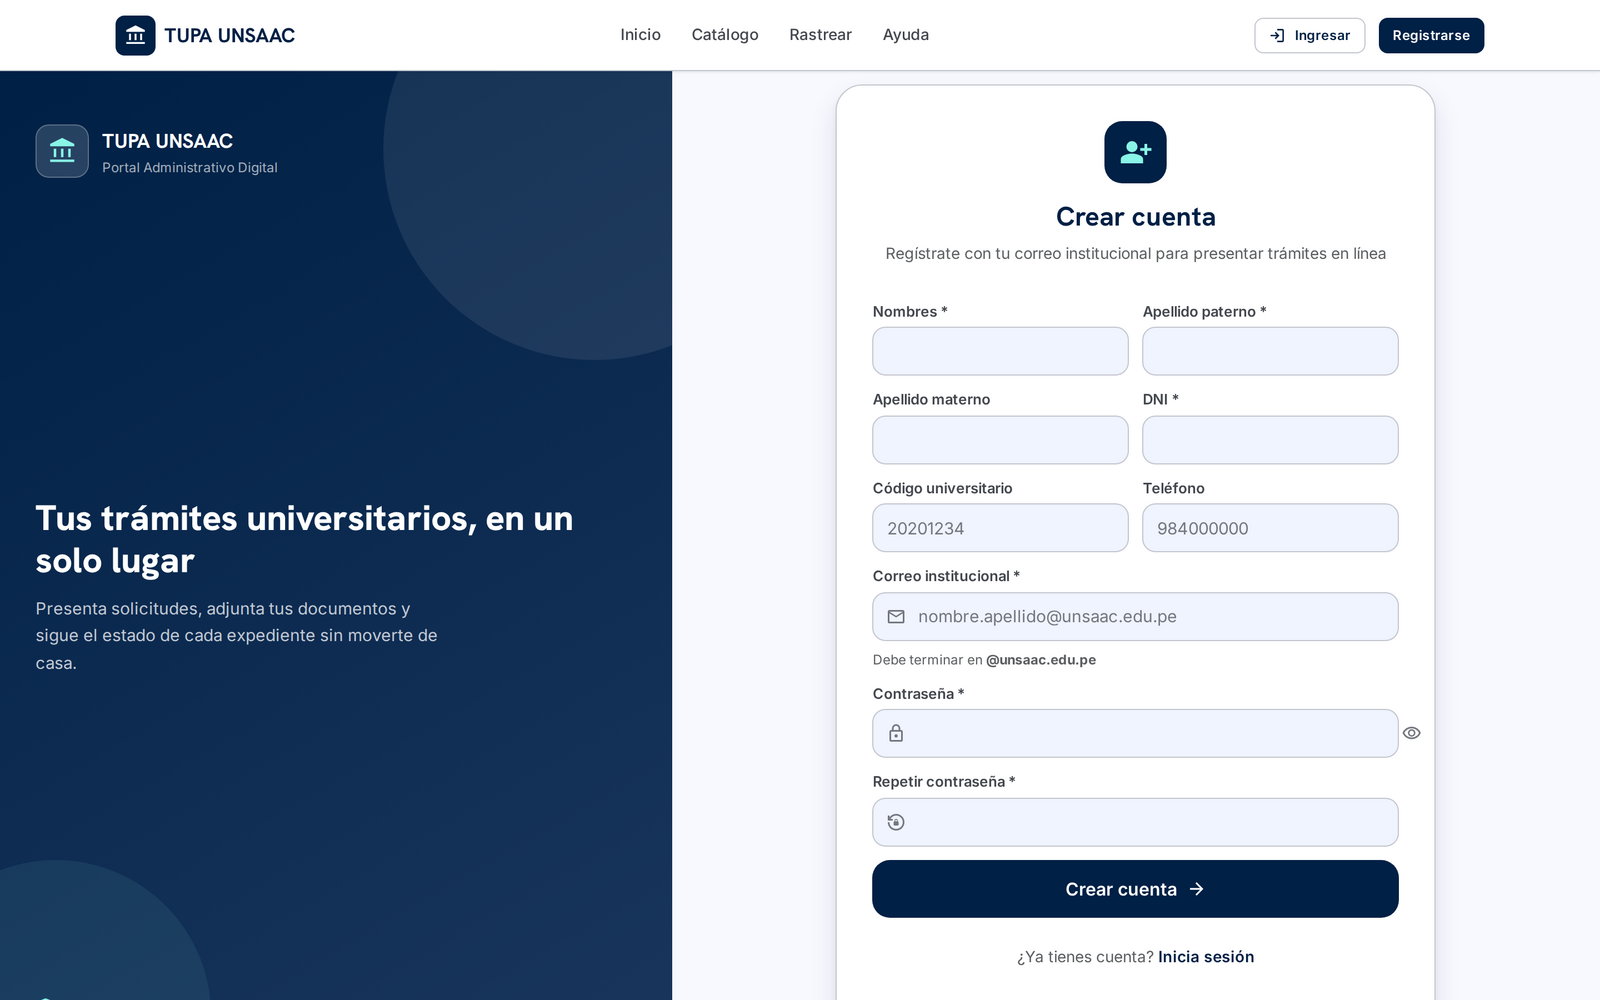
\includegraphics[width=0.95\textwidth]{images/capt-registro.png}}%
{Registro de cuenta con validación de correo institucional (ruta \texttt{/registro}).}{fig:registro}

\apafigure{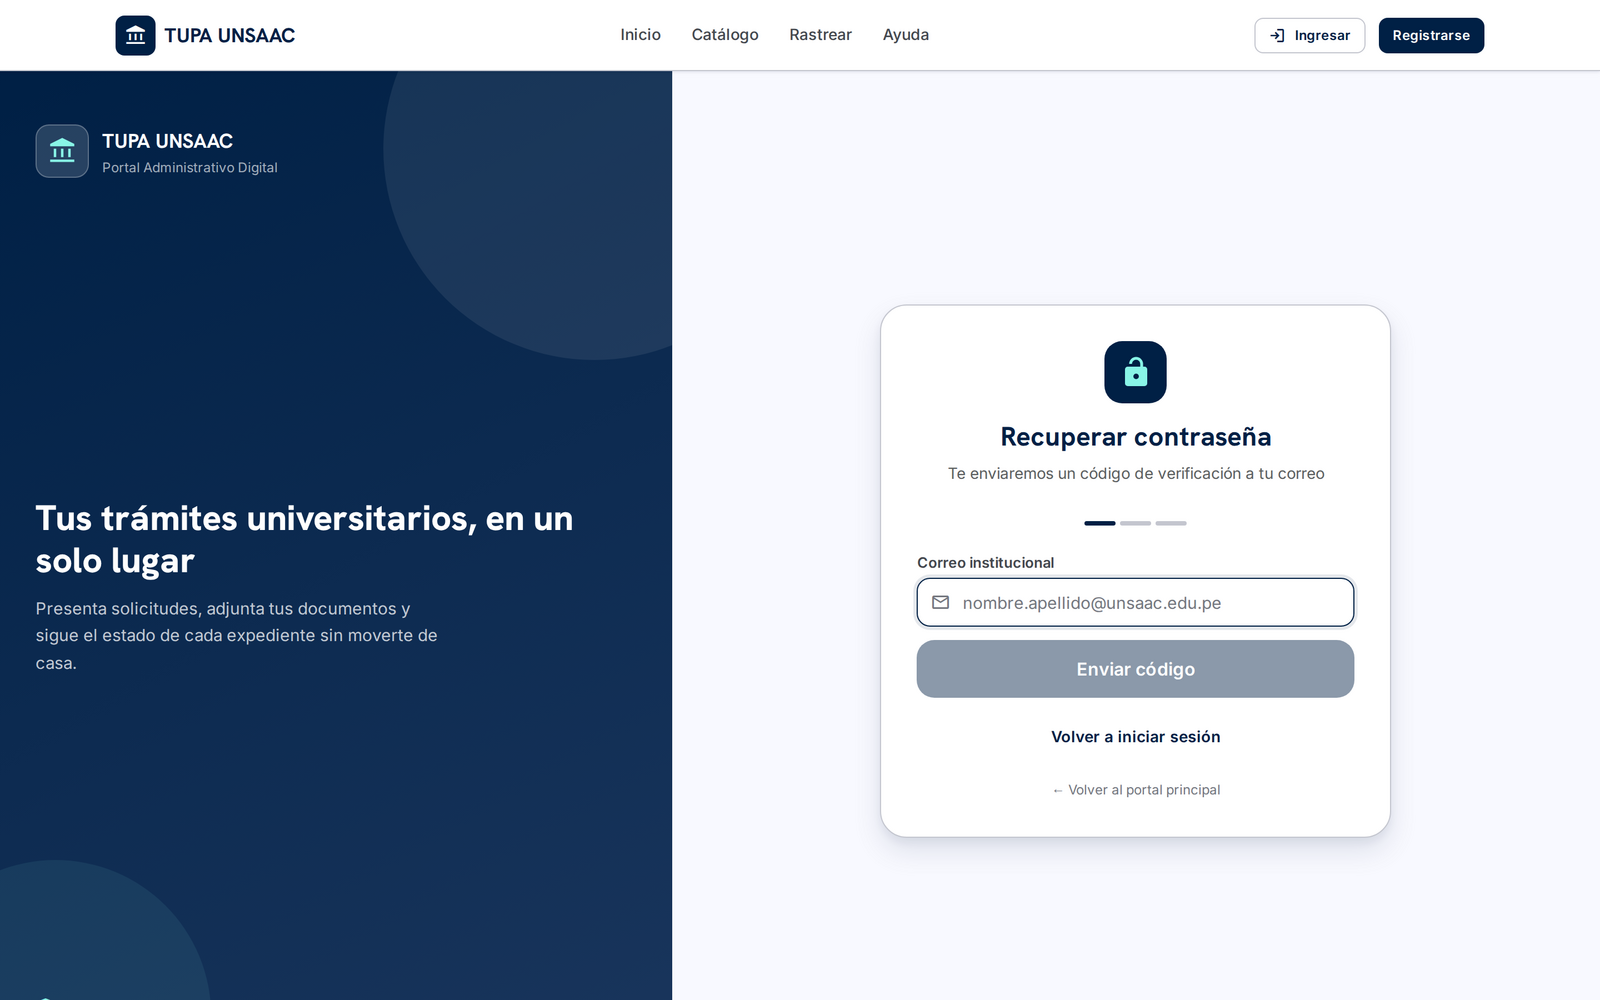
\includegraphics[width=0.95\textwidth]{images/capt-recuperar-password.png}}%
{Recuperación de contraseña mediante código de verificación (ruta \texttt{/recuperar-password}).}{fig:recuperar}

\apafigure{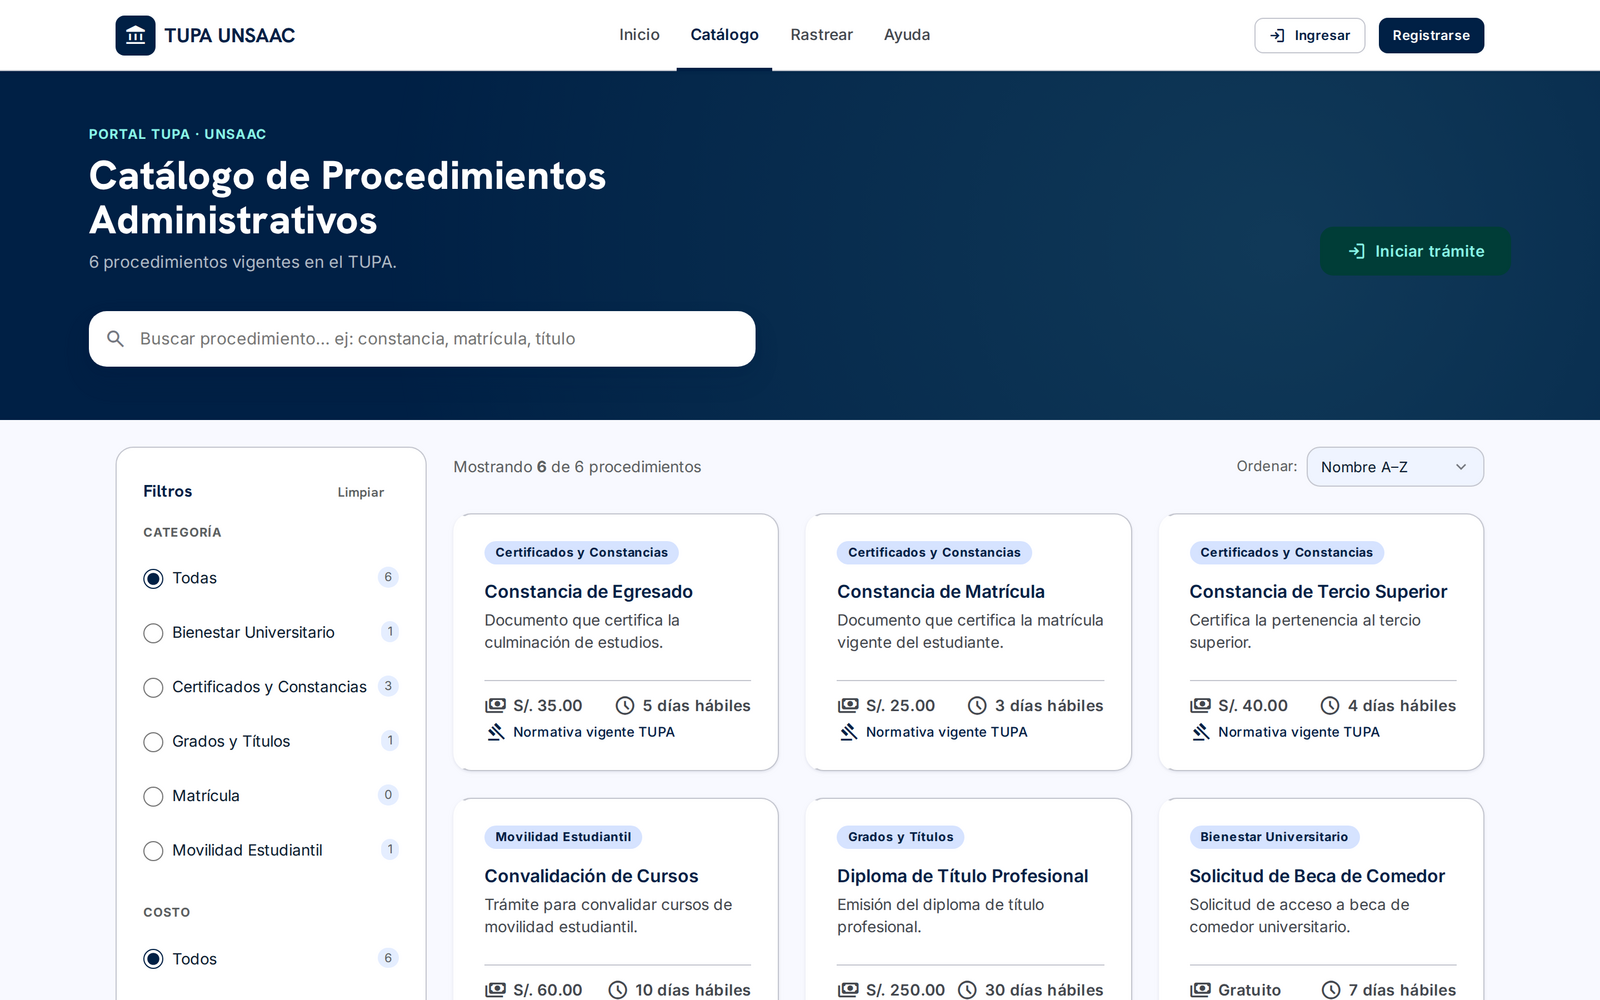
\includegraphics[width=0.95\textwidth]{images/capt-catalogo.png}}%
{Catálogo público de trámites del TUPA (ruta \texttt{/catalogo}).}{fig:catalogo}

\apafigure{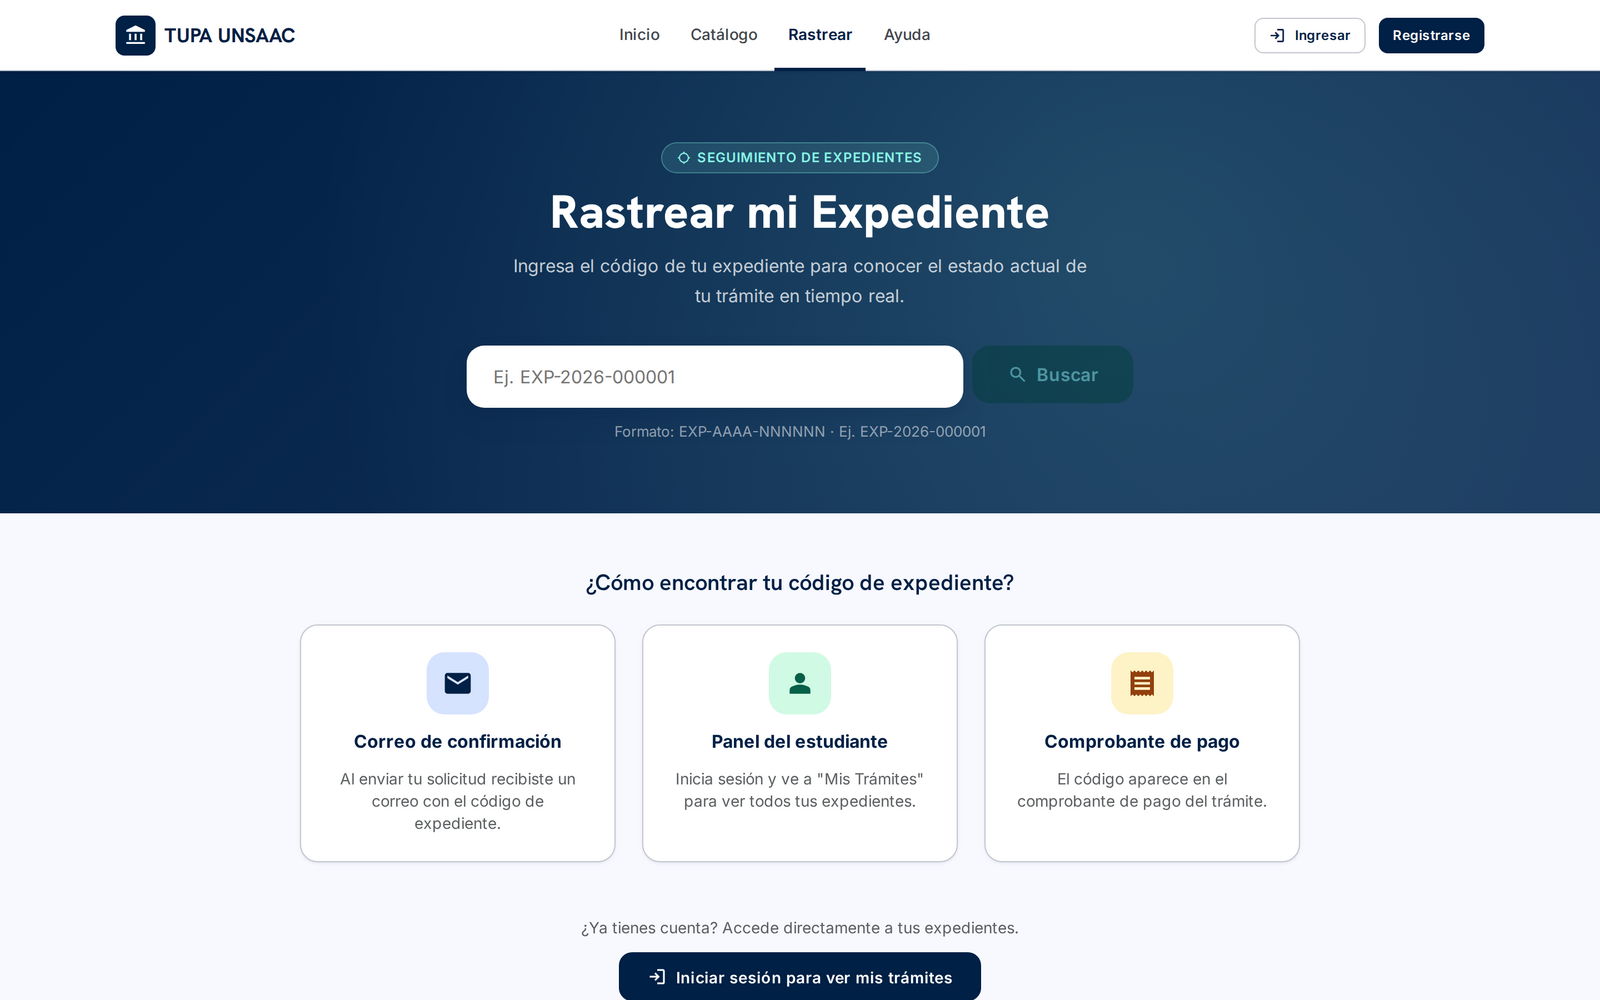
\includegraphics[width=0.95\textwidth]{images/capt-seguimiento-busqueda.png}}%
{Consulta pública de expediente (ruta \texttt{/seguimiento}).}{fig:seguimiento-busqueda}

\apafigure{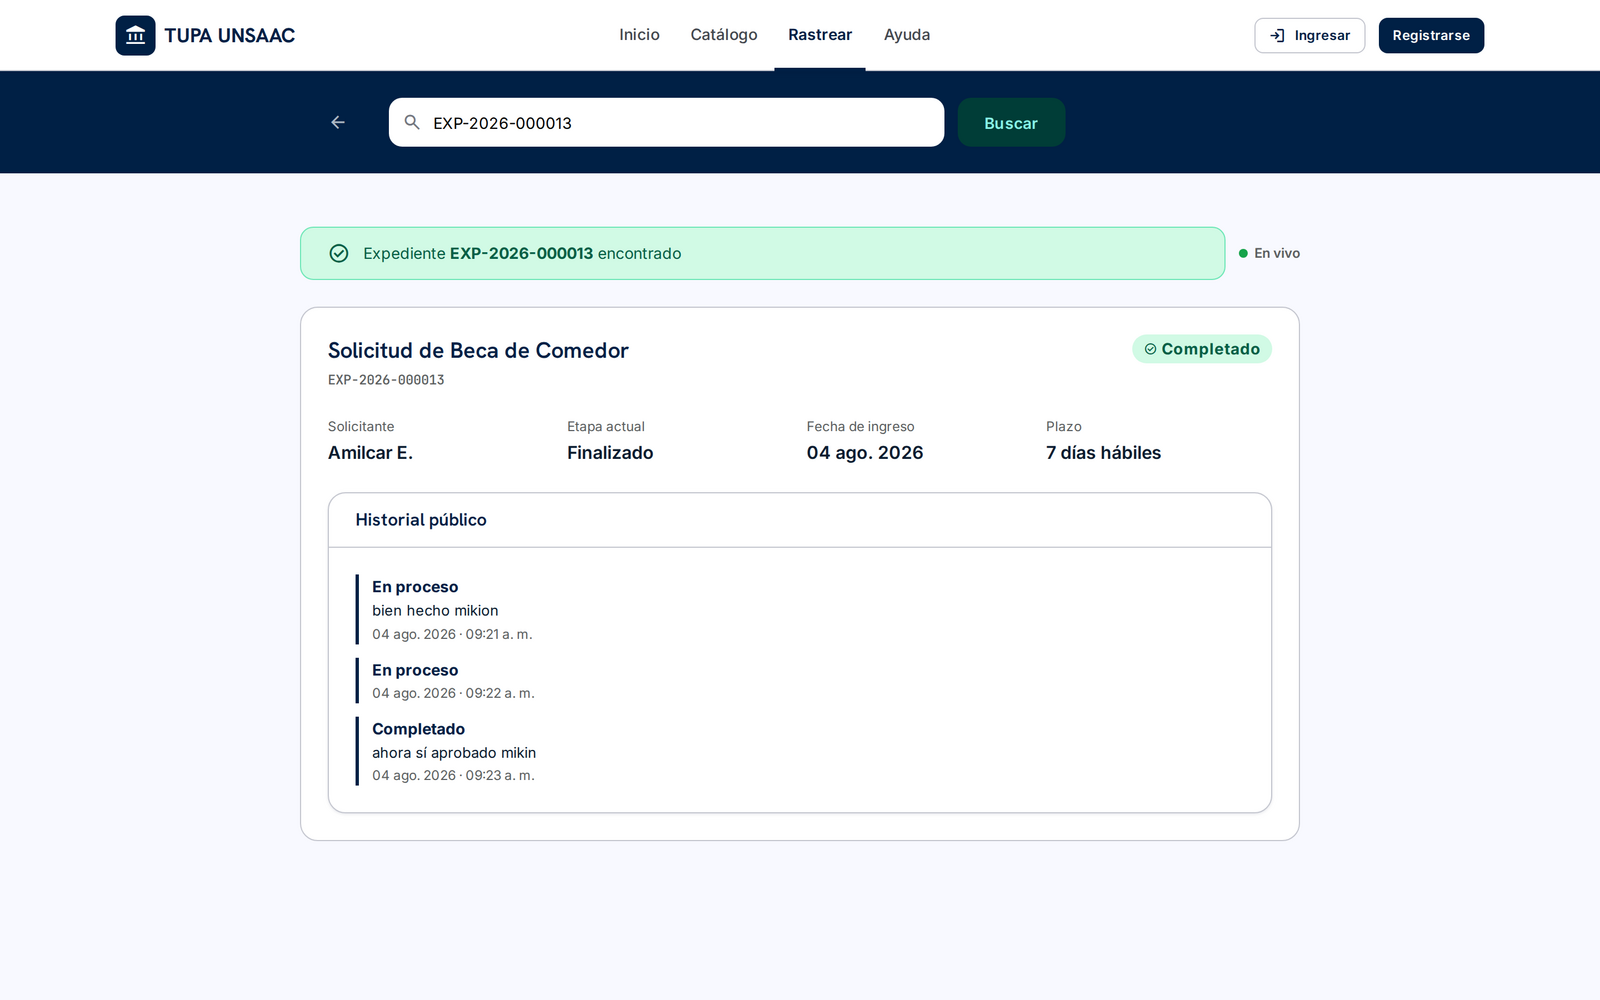
\includegraphics[width=0.95\textwidth]{images/capt-seguimiento-resultados.png}}%
{Resultado de la consulta pública, con el nombre del solicitante abreviado (ruta \texttt{/seguimiento/resultados}).}{fig:seguimiento-resultados}

\apafigure{%

\includegraphics[width=0.95\linewidth]{images/portal-inicio.png}%
}{Página de inicio del portal público, con acceso al catálogo, al seguimiento de expedientes y al ingreso al sistema.}{fig:portal-inicio}

\apafigure{%
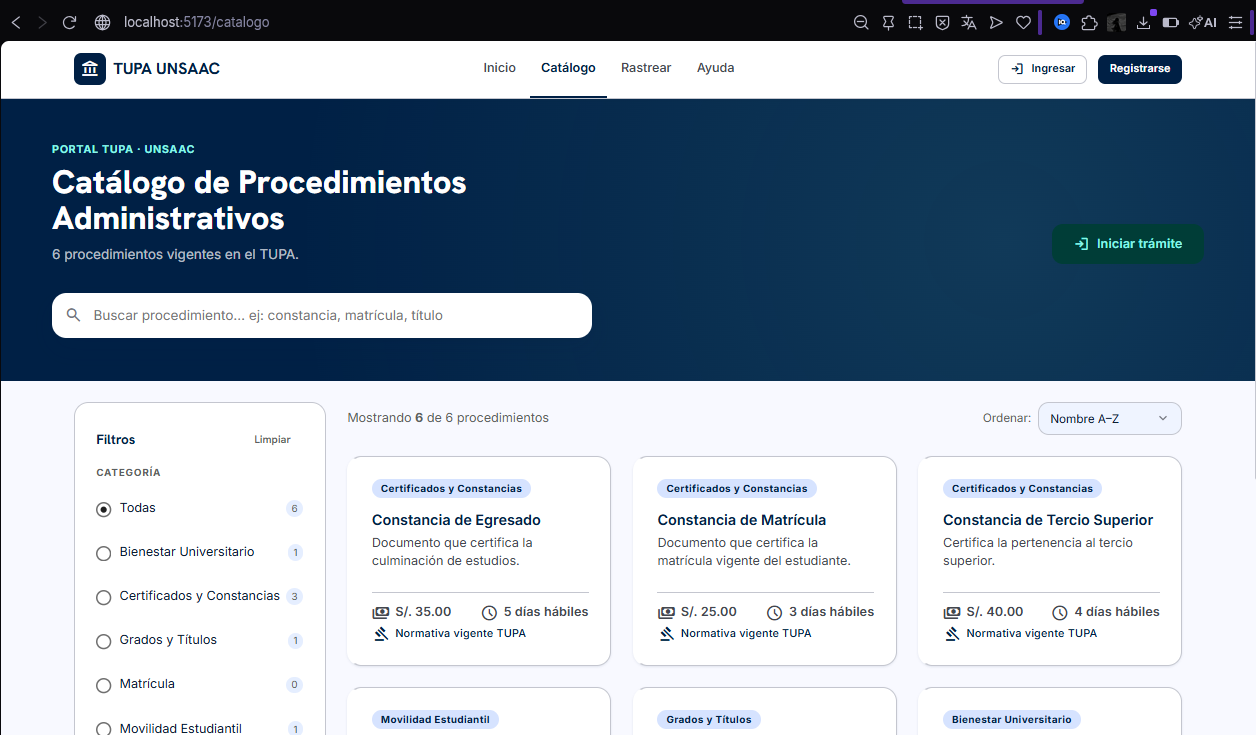
\includegraphics[width=0.95\linewidth]{images/catalogo-tramites.png}%
}{Catálogo de procedimientos administrativos, con buscador y filtros por categoría, costo y plazo.}{fig:catalogo-tramites}

\apafigure{%
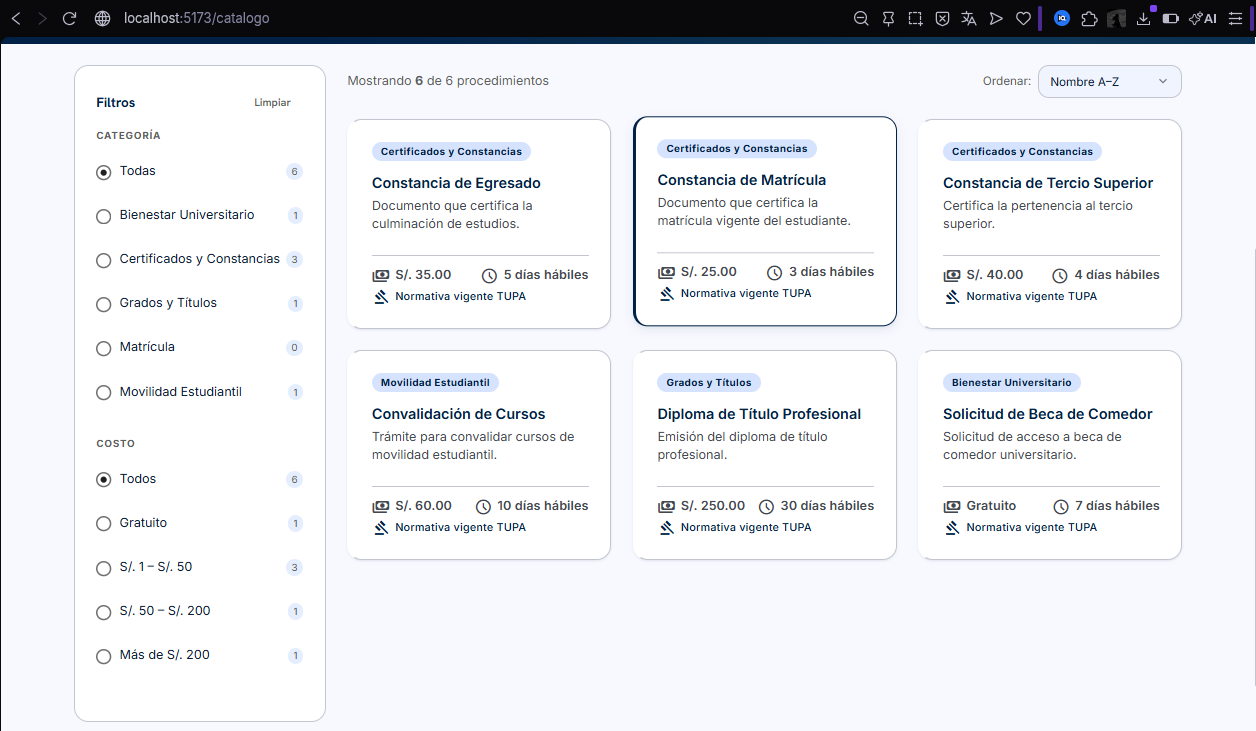
\includegraphics[width=0.95\linewidth]{images/catalogo-filtros.png}%
}{Listado de trámites del catálogo filtrado por categoría y rango de costo.}{fig:catalogo-filtros}

\apafigure{%
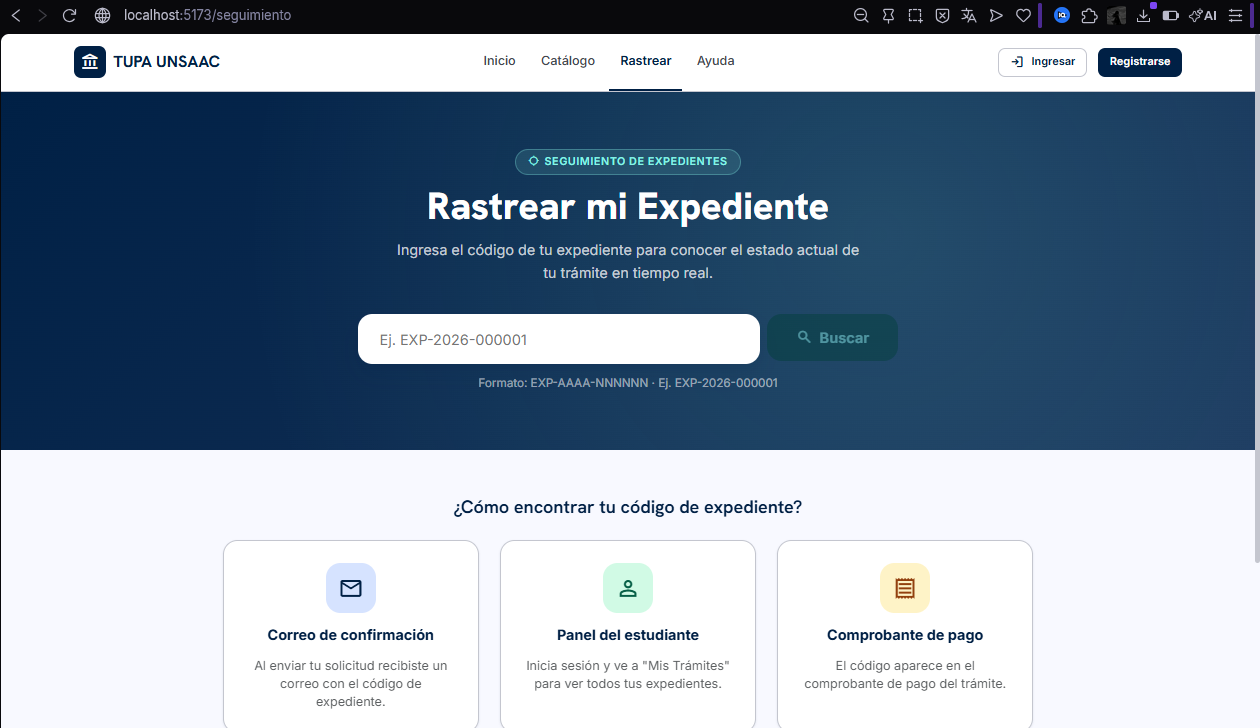
\includegraphics[width=0.95\linewidth]{images/rastreo-expediente.png}%
}{Vista pública de rastreo de expediente por número de código.}{fig:rastreo-expediente}

\apafigure{%
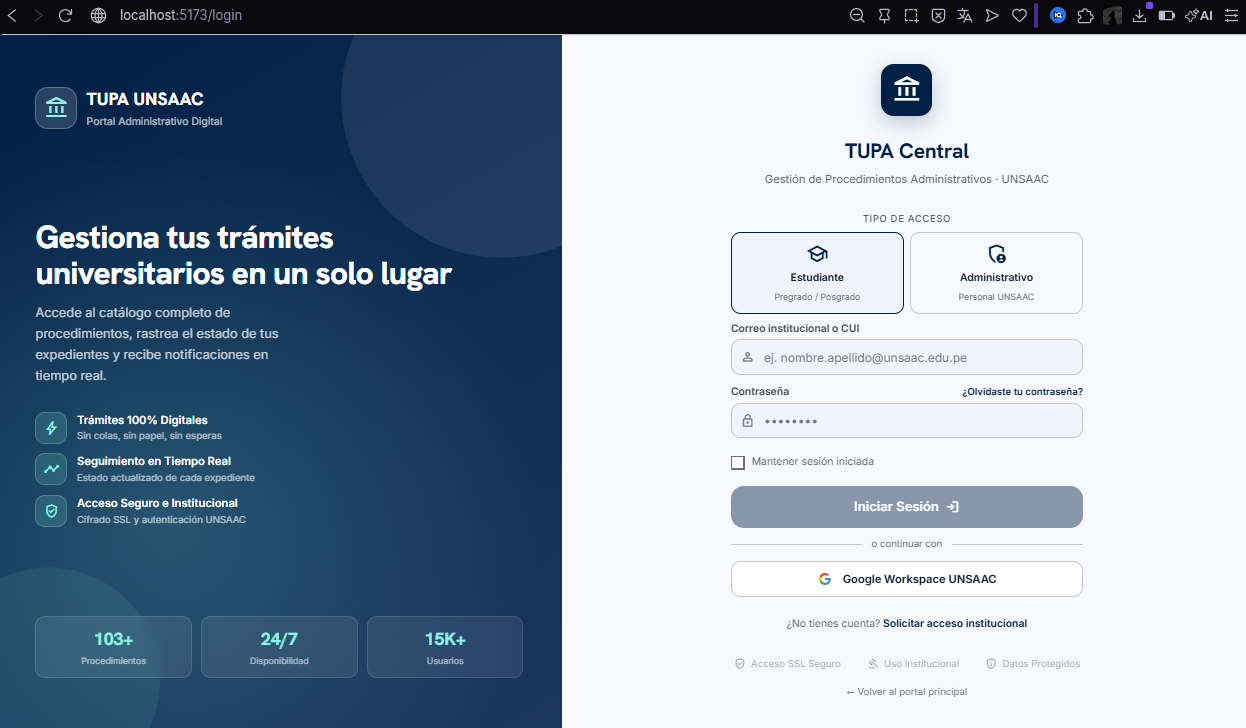
\includegraphics[width=0.95\linewidth]{images/login.png}%
}{Pantalla de inicio de sesión, con selección de tipo de acceso (estudiante o administrativo).}{fig:login}

\subsubsection{Portal del Estudiante}
El portal del estudiante incorpora el tablero principal, el perfil, el centro
de notificaciones, el listado de trámites y solicitudes y el detalle de cada
expediente. En la estructura del frontend, estos módulos se materializan en
\texttt{Dashboard.jsx}, \texttt{MyProfile.jsx}, \texttt{Notifications.jsx},
\texttt{MyProcedures.jsx}, \texttt{MyRequests.jsx} y \texttt{RequestDetail.jsx}.

\apafigure{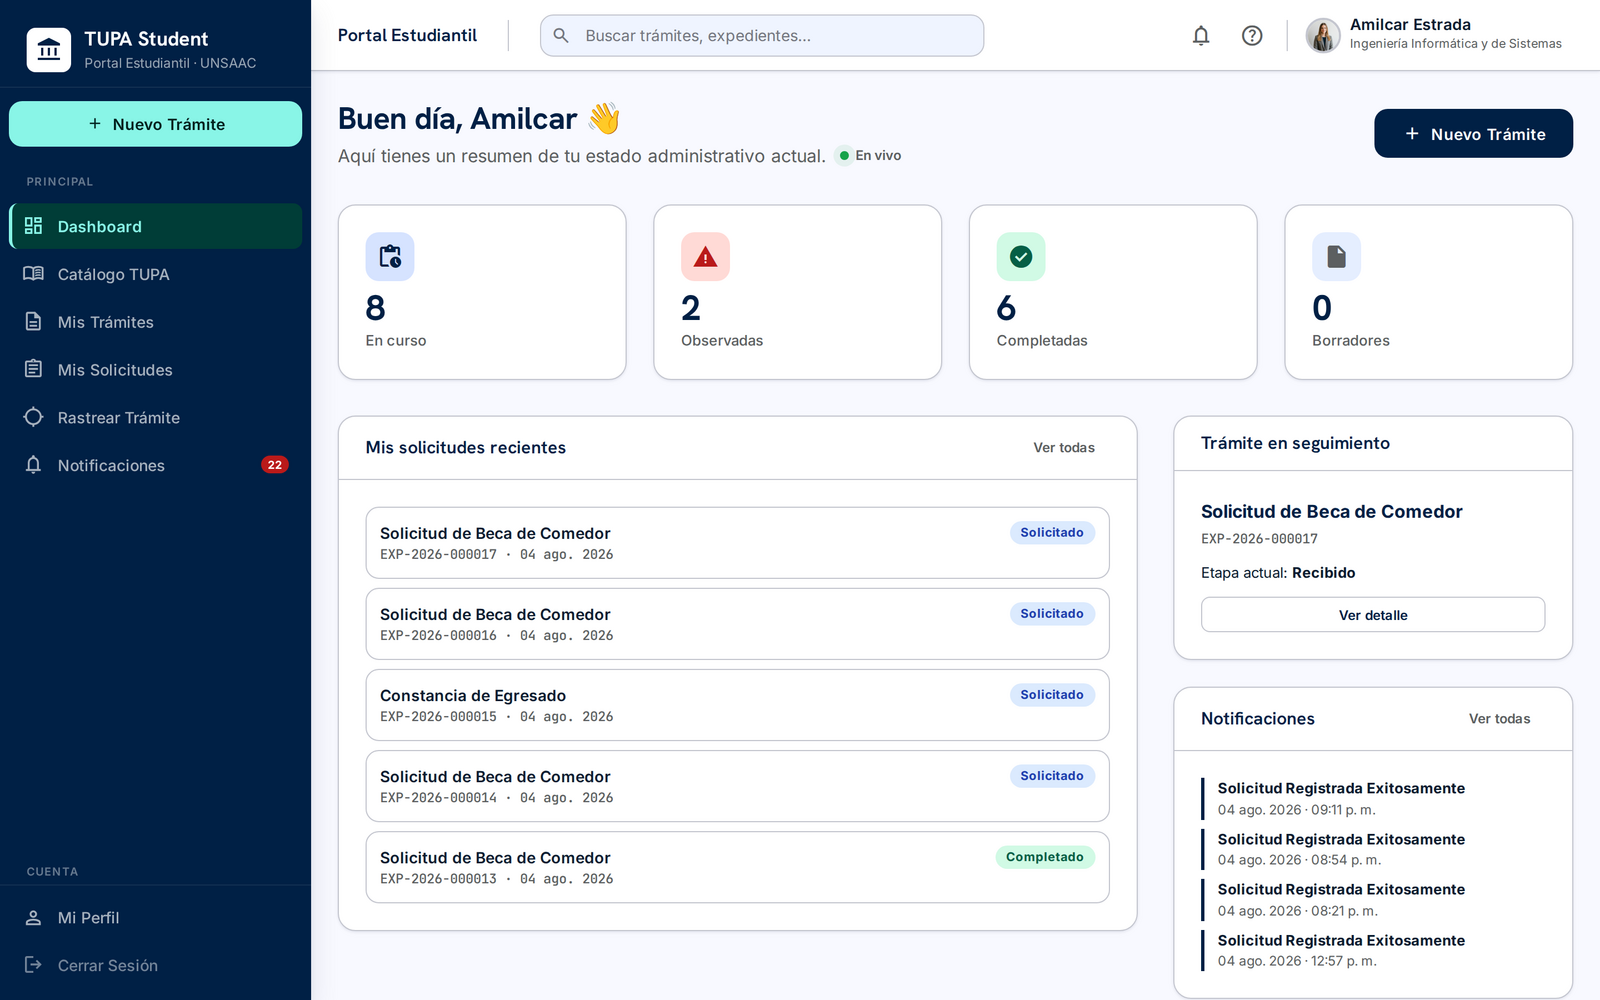
\includegraphics[width=0.95\textwidth]{images/capt-est-dashboard.png}}%
{Tablero principal del estudiante (ruta \texttt{/estudiante}).}{fig:est-dashboard}

\apafigure{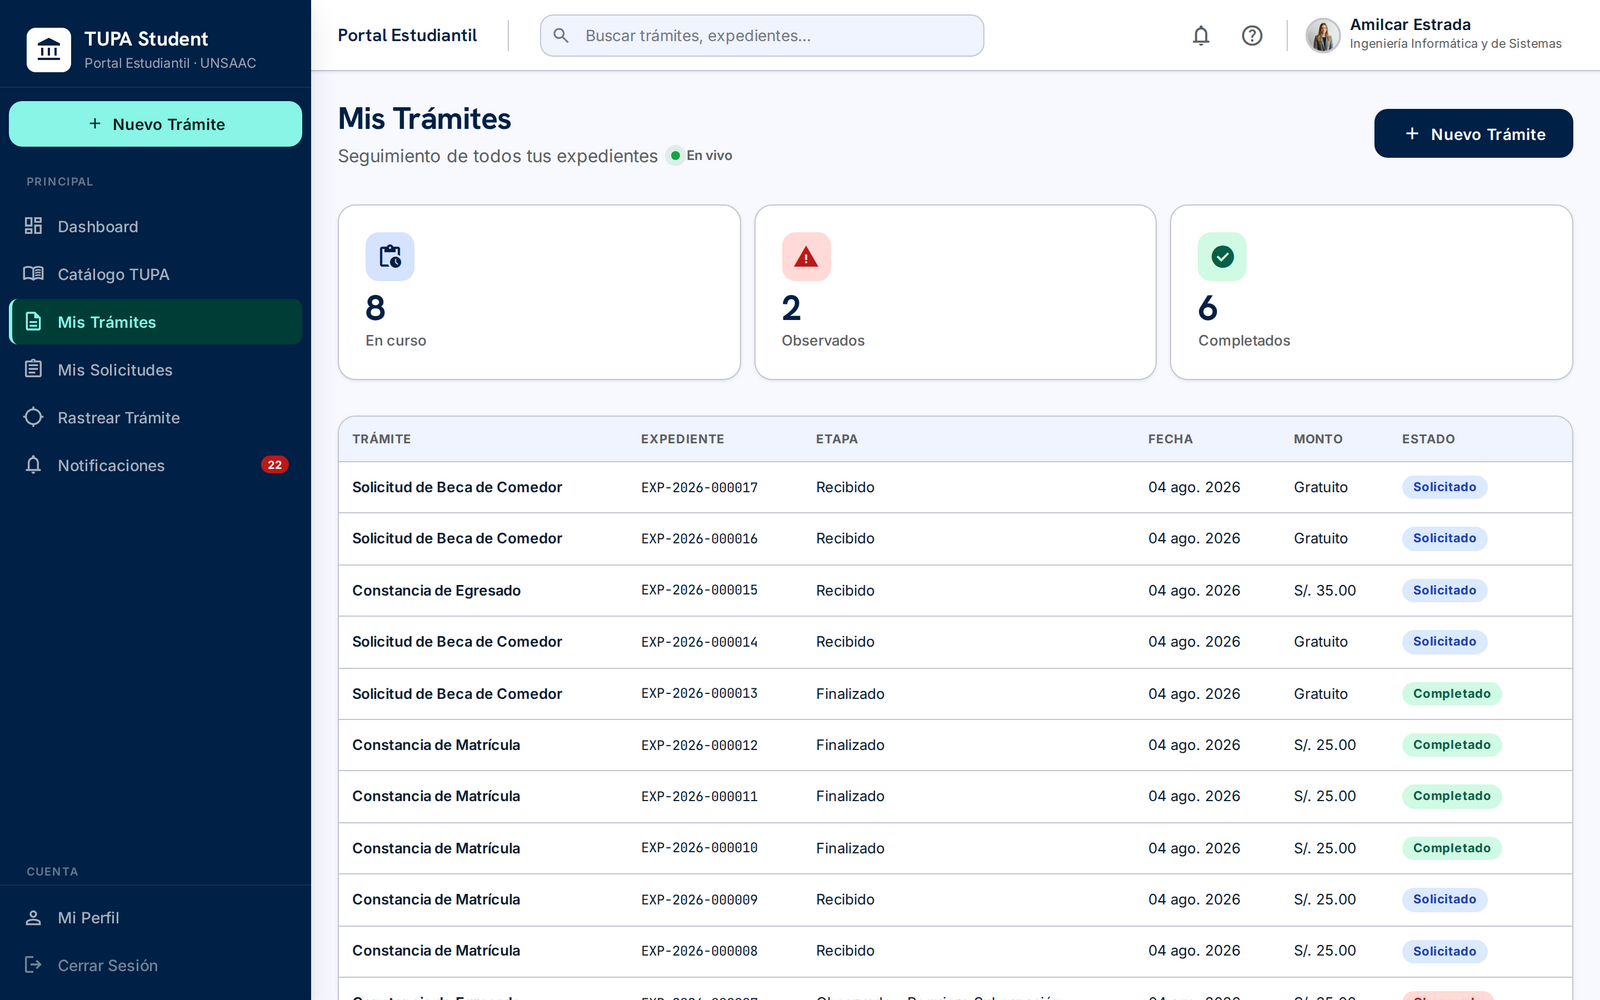
\includegraphics[width=0.95\textwidth]{images/capt-est-tramites.png}}%
{Catálogo de trámites disponibles dentro del portal del estudiante (ruta \texttt{/estudiante/tramites}).}{fig:est-tramites}

\apafigure{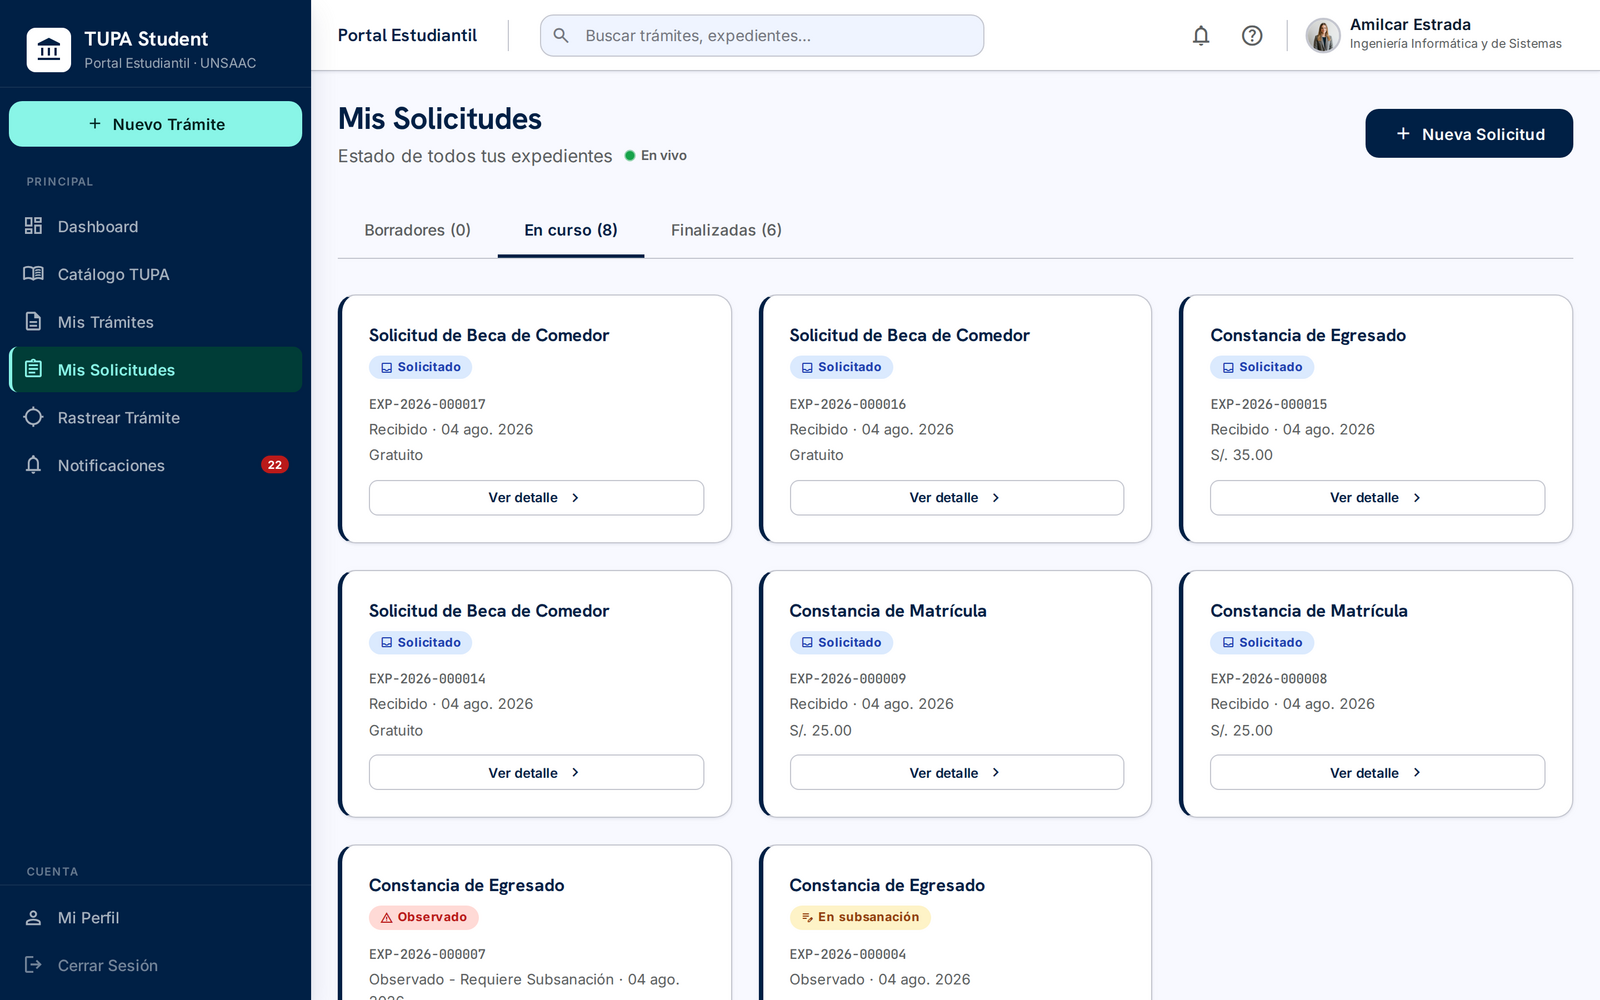
\includegraphics[width=0.95\textwidth]{images/capt-est-solicitudes.png}}%
{Listado de solicitudes del estudiante con su estado actual (ruta \texttt{/estudiante/solicitudes}).}{fig:est-solicitudes}

\apafigure{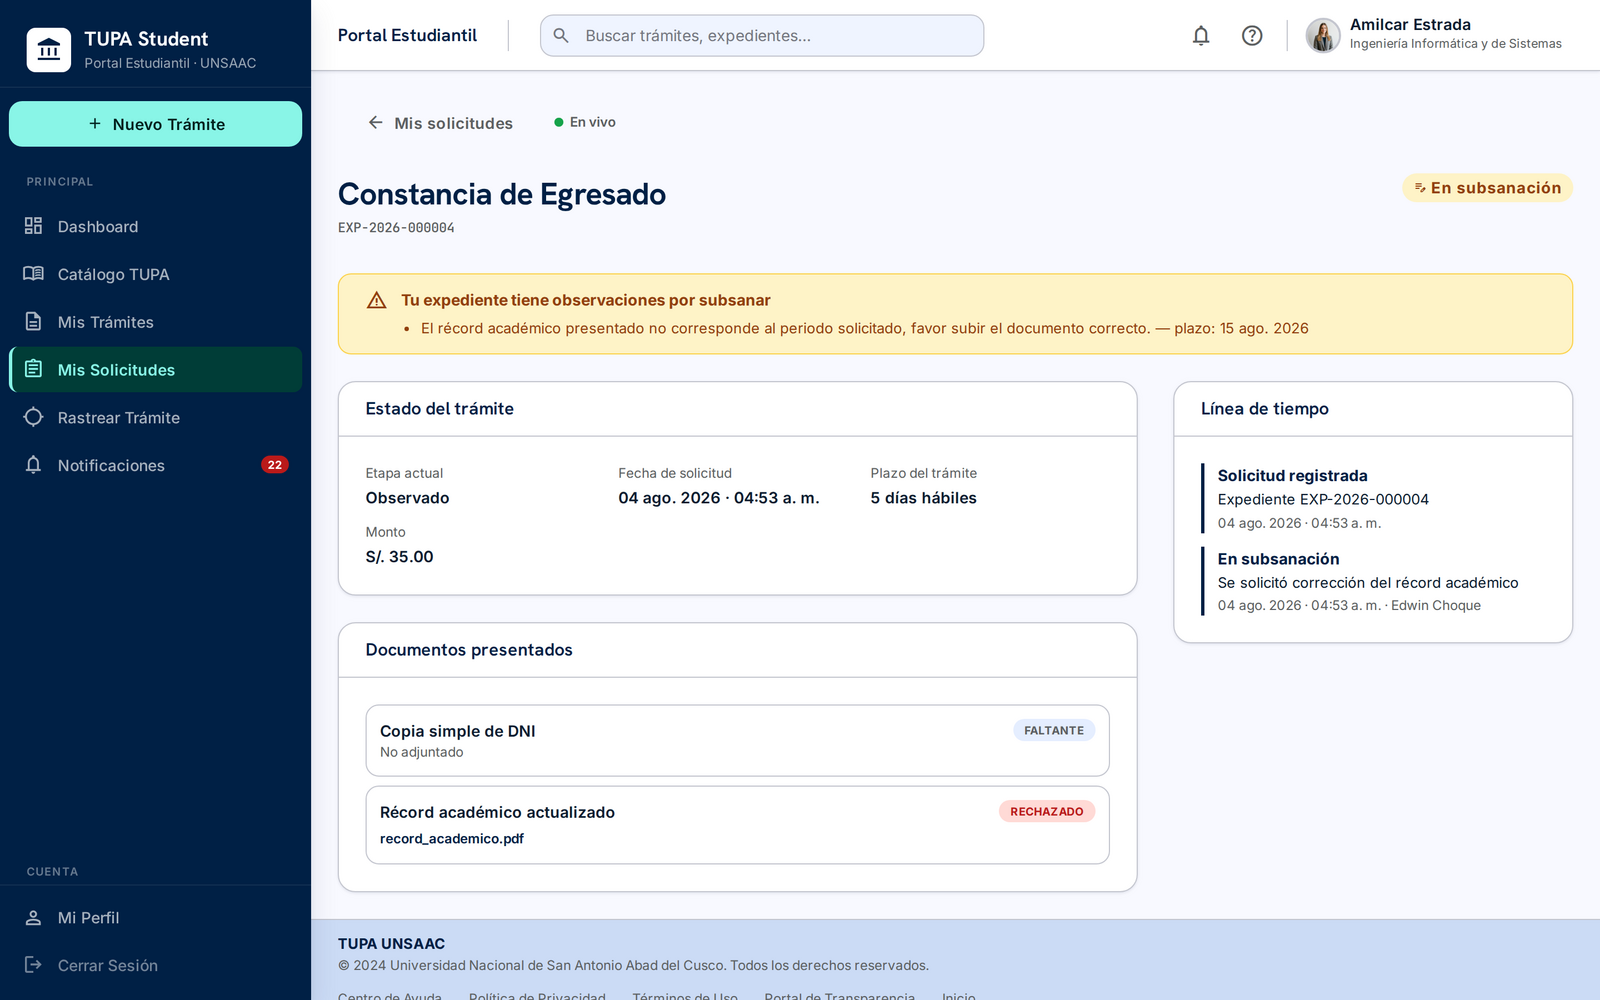
\includegraphics[width=0.95\textwidth]{images/capt-est-solicitud-detalle.png}}%
{Detalle de un expediente en subsanación, con observaciones, documentos y línea de tiempo (ruta \texttt{/estudiante/solicitudes/:id}).}{fig:est-solicitud-detalle}

\apafigure{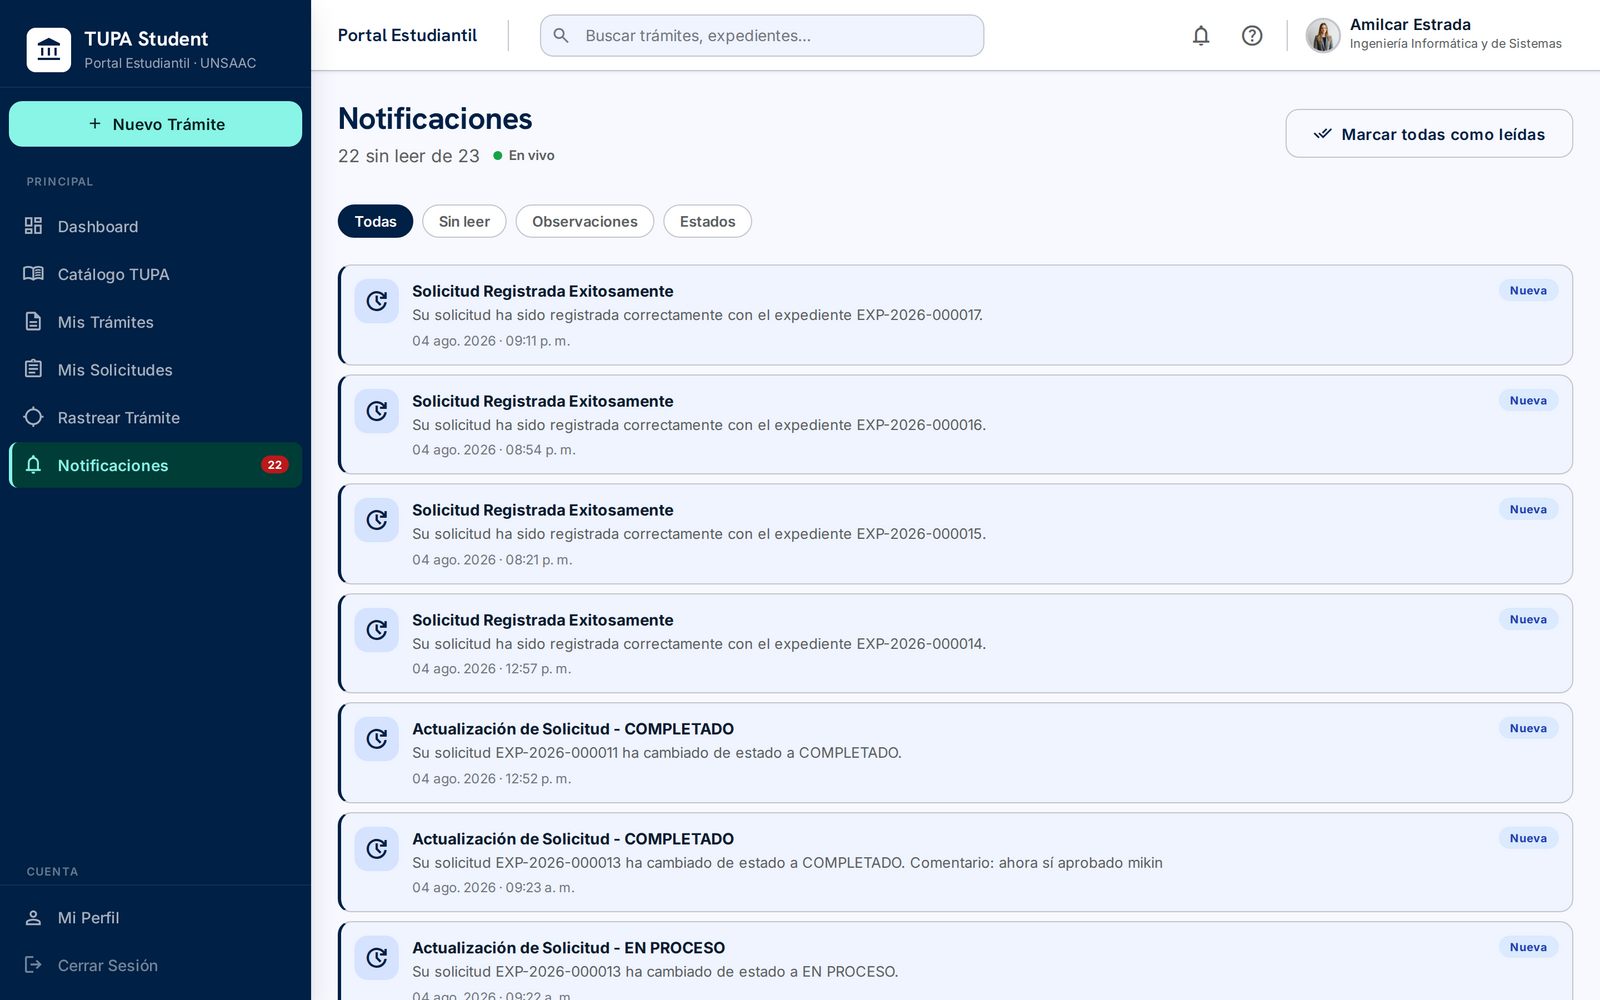
\includegraphics[width=0.95\textwidth]{images/capt-est-notificaciones.png}}%
{Centro de notificaciones del estudiante (ruta \texttt{/estudiante/notificaciones}).}{fig:est-notificaciones}

\apafigure{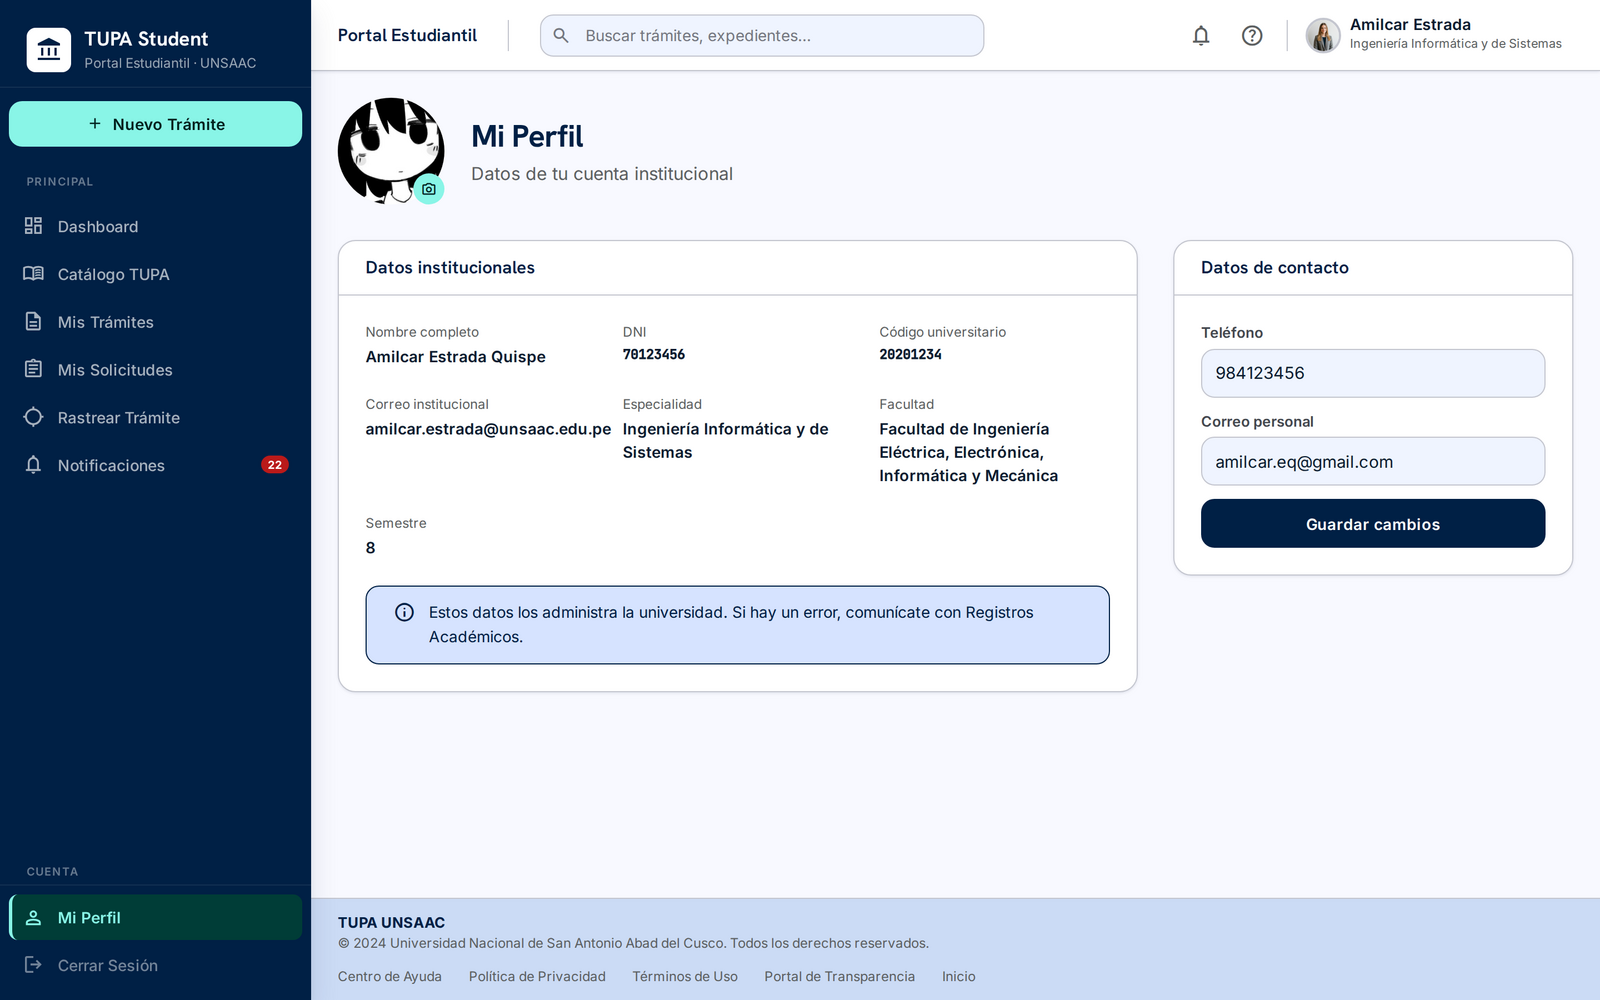
\includegraphics[width=0.95\textwidth]{images/capt-est-perfil.png}}%
{Perfil del estudiante; sólo los datos de contacto son editables (ruta \texttt{/estudiante/perfil}).}{fig:est-perfil}

\subsubsection{Asistente de Solicitud}
El envío de una solicitud se realiza mediante un asistente de seis pasos
(\texttt{wizard/Step1.jsx} a \texttt{Step6.jsx}), cuyo estado se comparte
entre rutas a través de \texttt{WizardContext}: selección del trámite,
revisión de requisitos, confirmación de pago, carga de documentos, revisión
final y confirmación de envío.

\apafigure{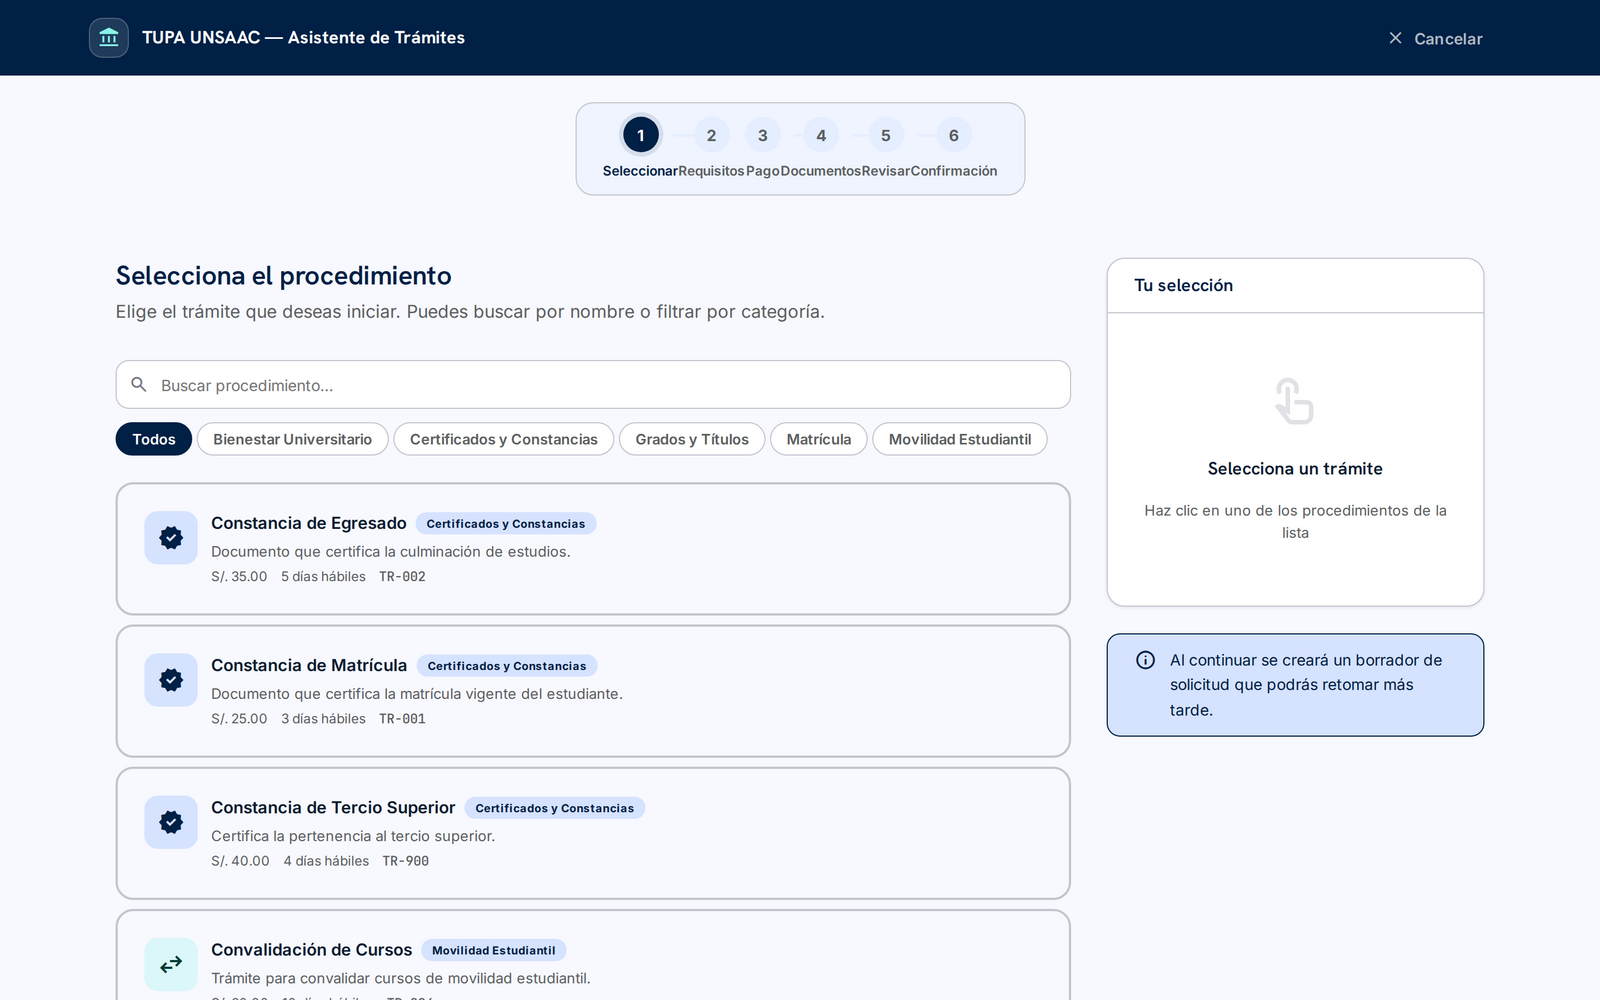
\includegraphics[width=0.95\textwidth]{images/capt-wizard-paso1.png}}%
{Paso 1 del asistente: selección del trámite (ruta \texttt{/tramite/paso1}).}{fig:wizard1}

\apafigure{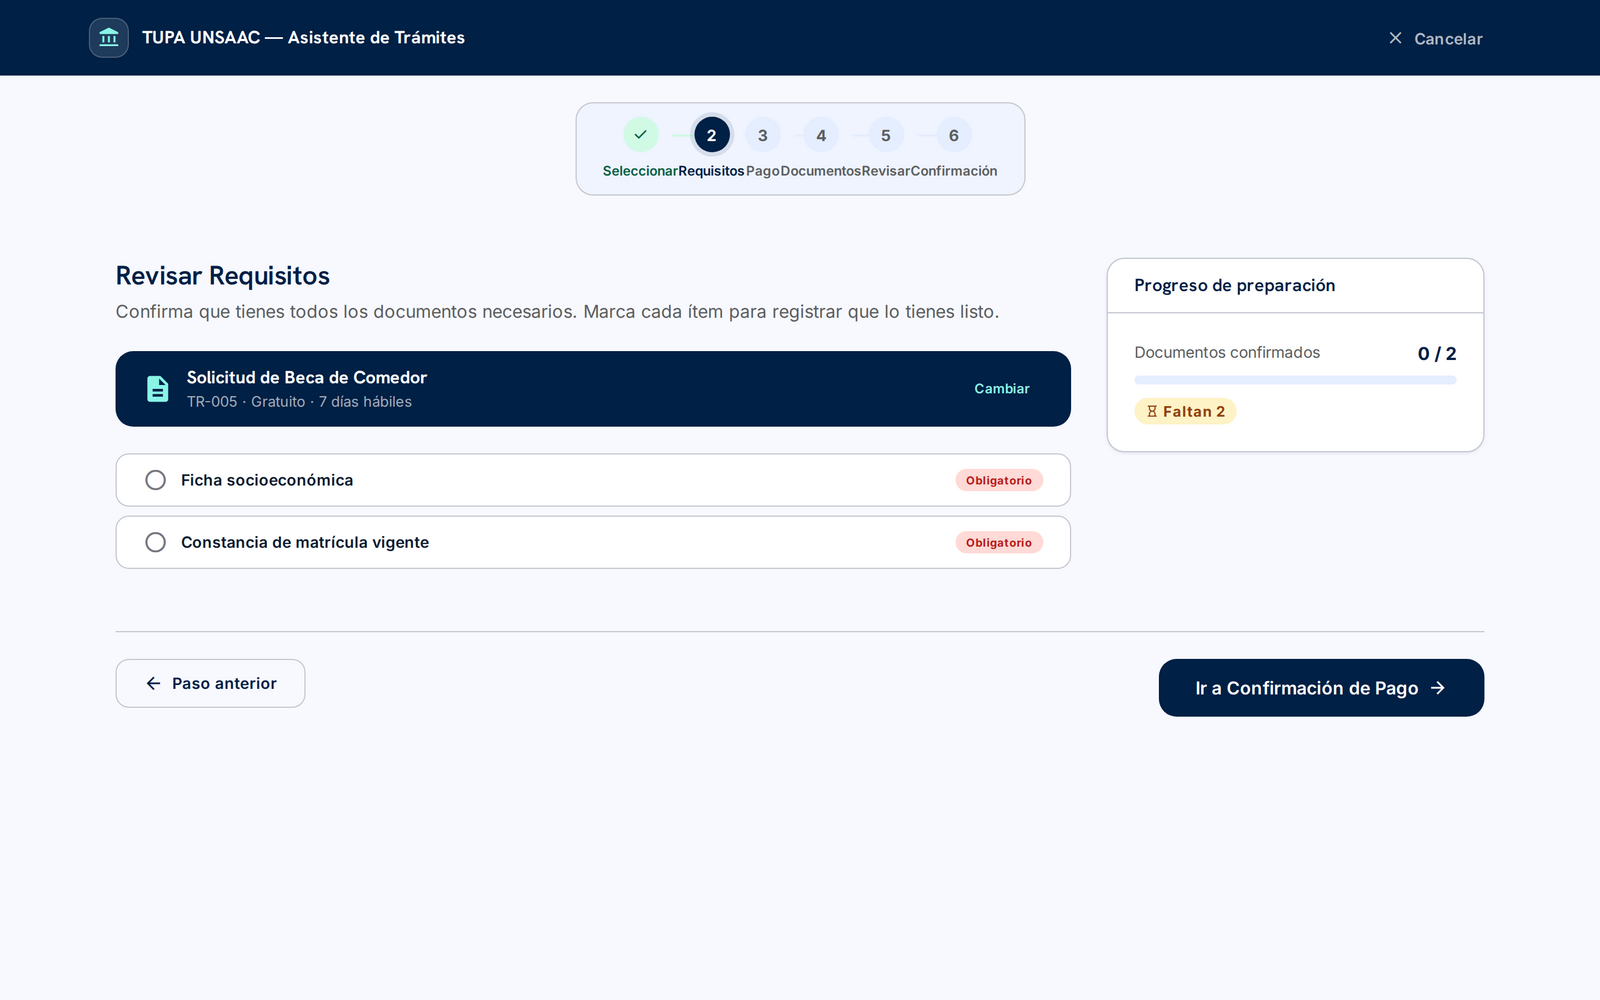
\includegraphics[width=0.95\textwidth]{images/capt-wizard-paso2.png}}%
{Paso 2 del asistente: revisión de requisitos del trámite elegido.}{fig:wizard2}

\apafigure{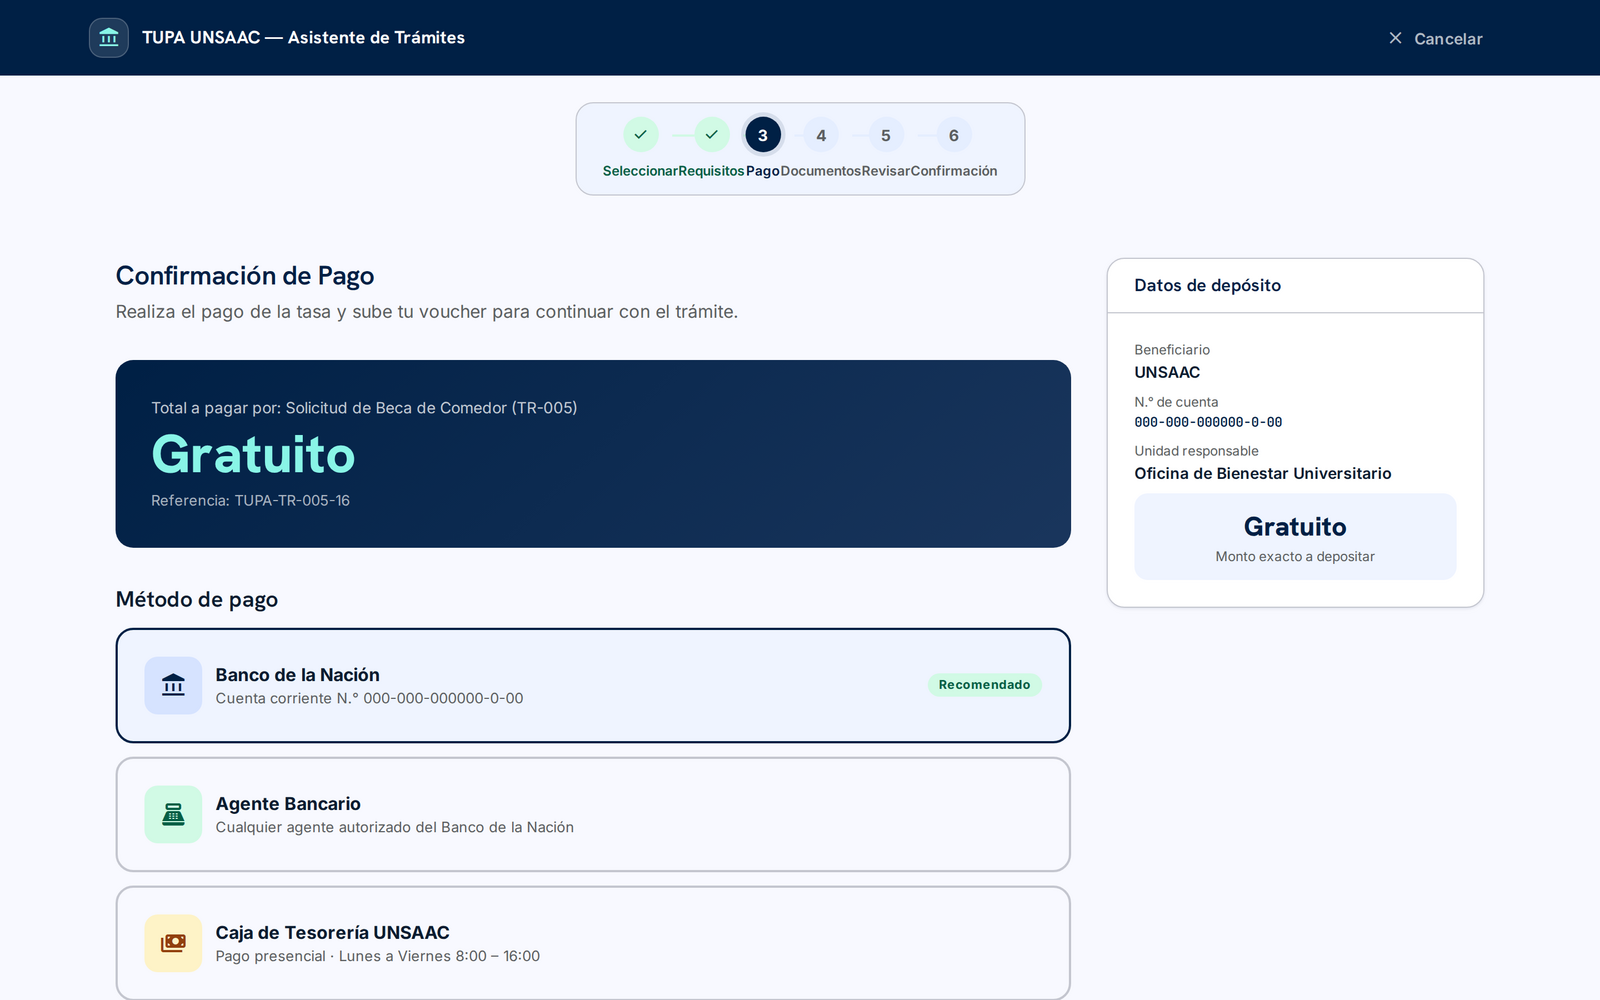
\includegraphics[width=0.95\textwidth]{images/capt-wizard-paso3.png}}%
{Paso 3 del asistente: confirmación de pago y carga del comprobante.}{fig:wizard3}

\apafigure{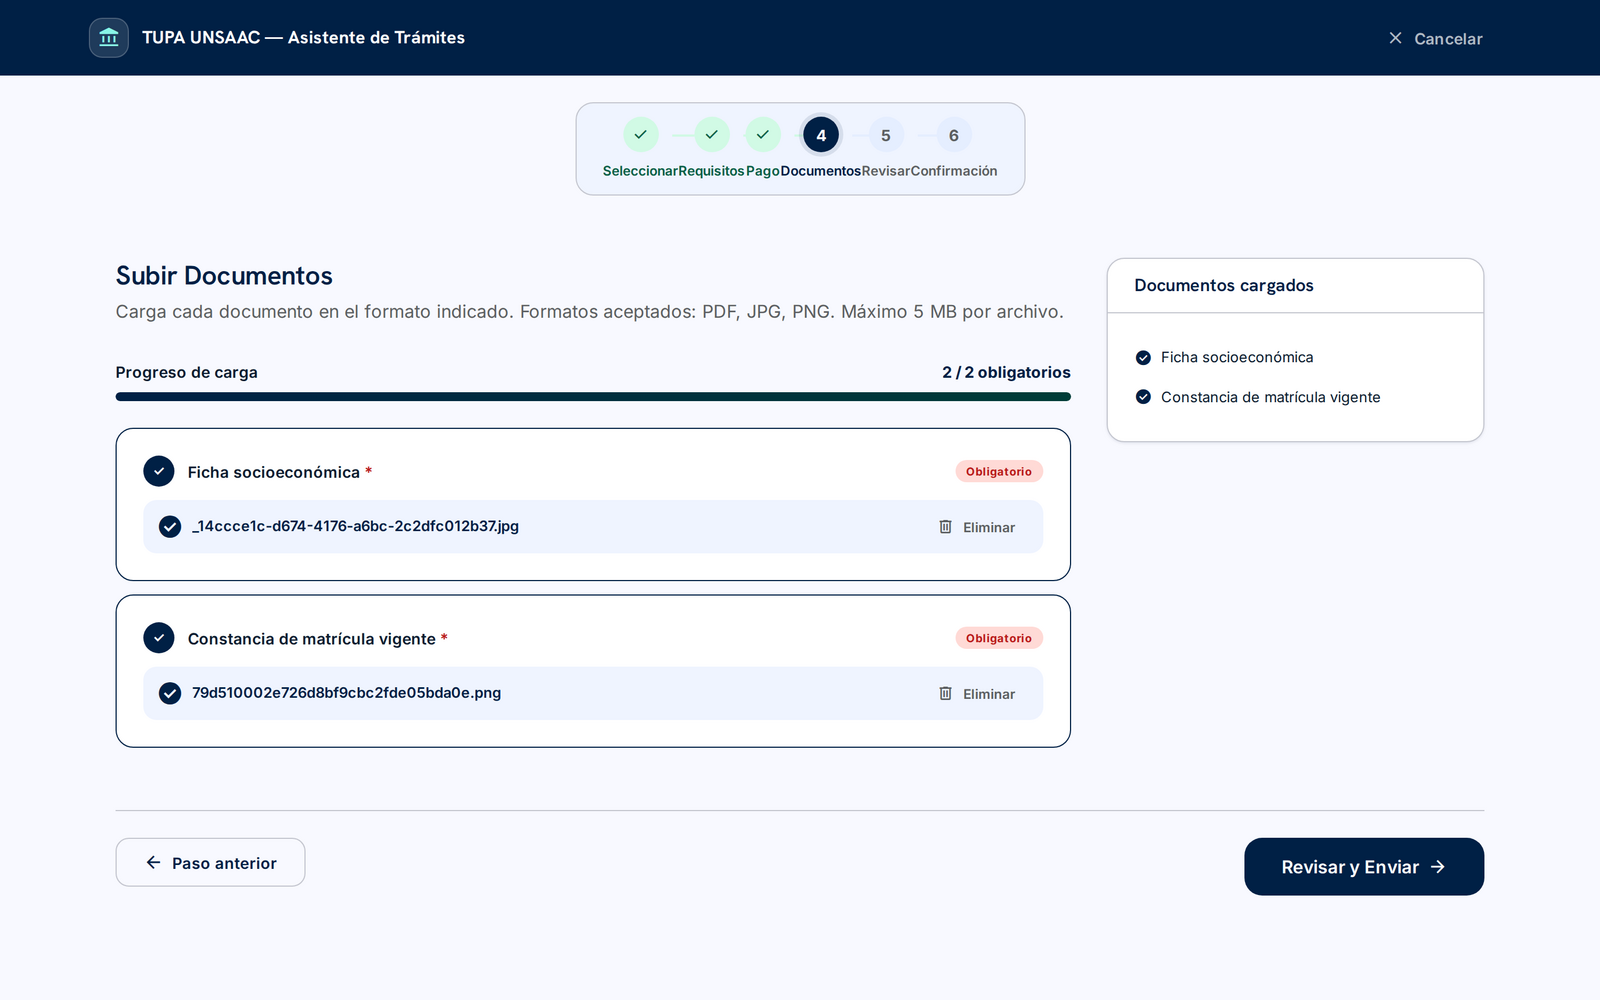
\includegraphics[width=0.95\textwidth]{images/capt-wizard-paso4.png}}%
{Paso 4 del asistente: carga de los documentos por requisito.}{fig:wizard4}

\apafigure{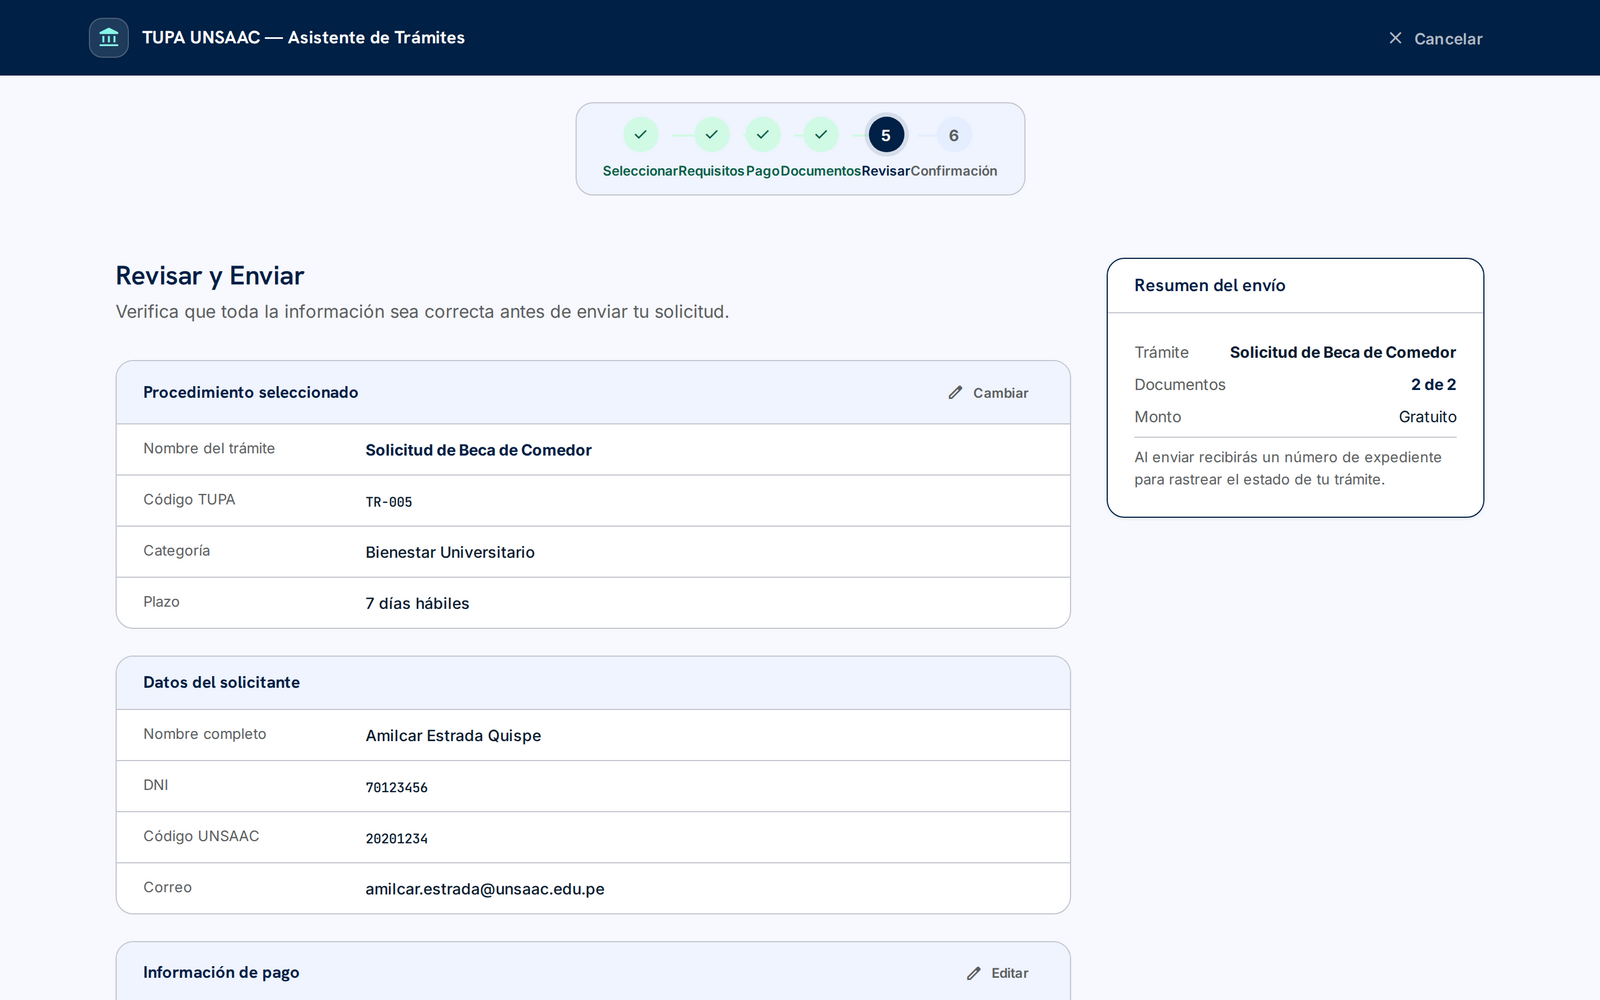
\includegraphics[width=0.95\textwidth]{images/capt-wizard-paso5.png}}%
{Paso 5 del asistente: revisión final antes del envío.}{fig:wizard5}

\apafigure{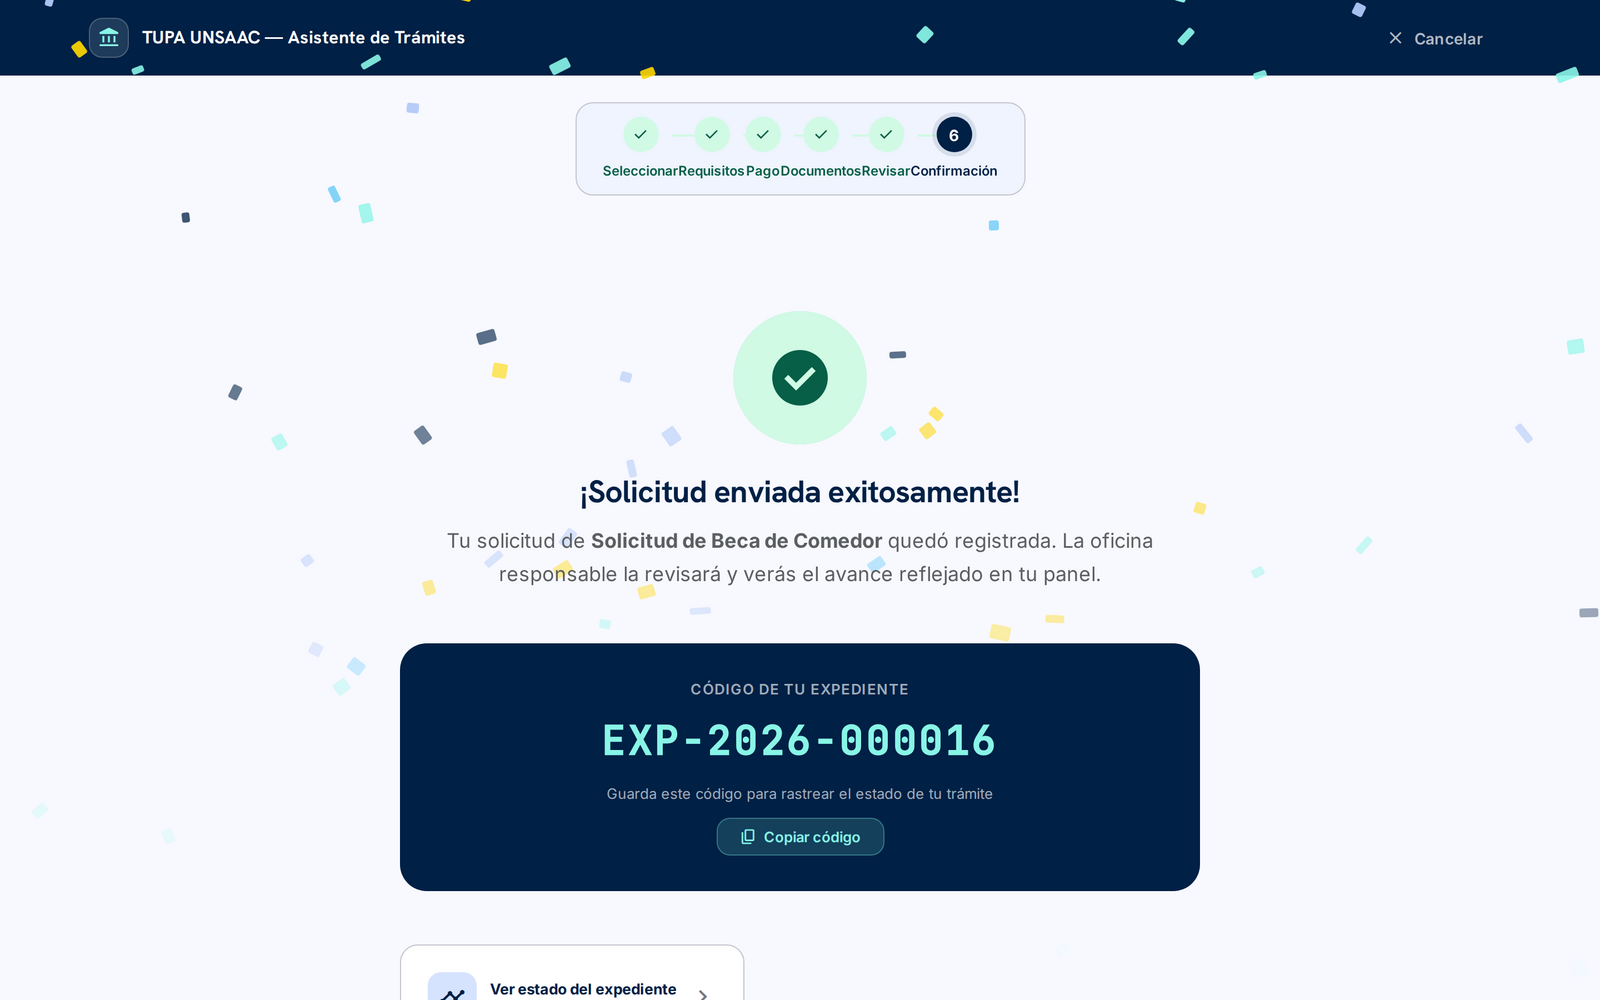
\includegraphics[width=0.95\textwidth]{images/capt-wizard-paso6.png}}%
{Paso 6 del asistente: confirmación de envío con el número de expediente generado.}{fig:wizard6}

\apafigure{%
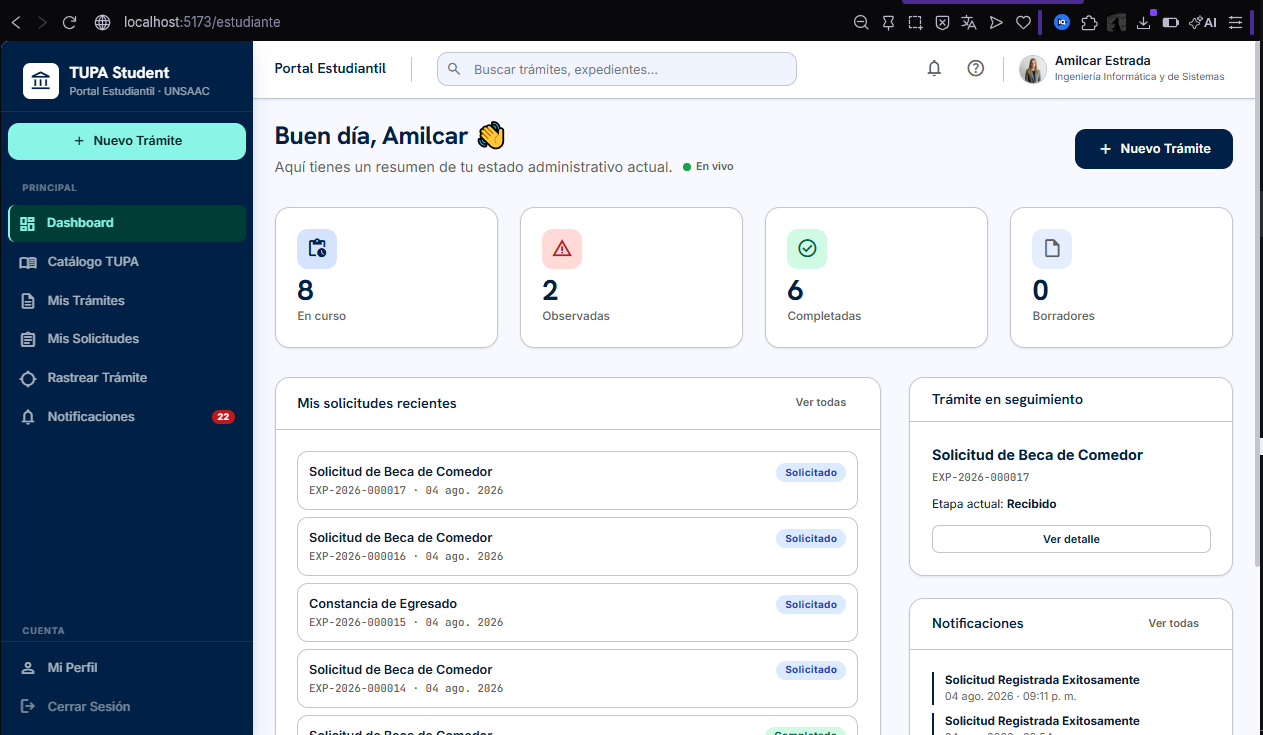
\includegraphics[width=0.95\linewidth]{images/estudiante-dashboard.png}%
}{Dashboard del estudiante, con el resumen de expedientes en curso, observados y completados.}{fig:estudiante-dashboard}

\apafigure{%
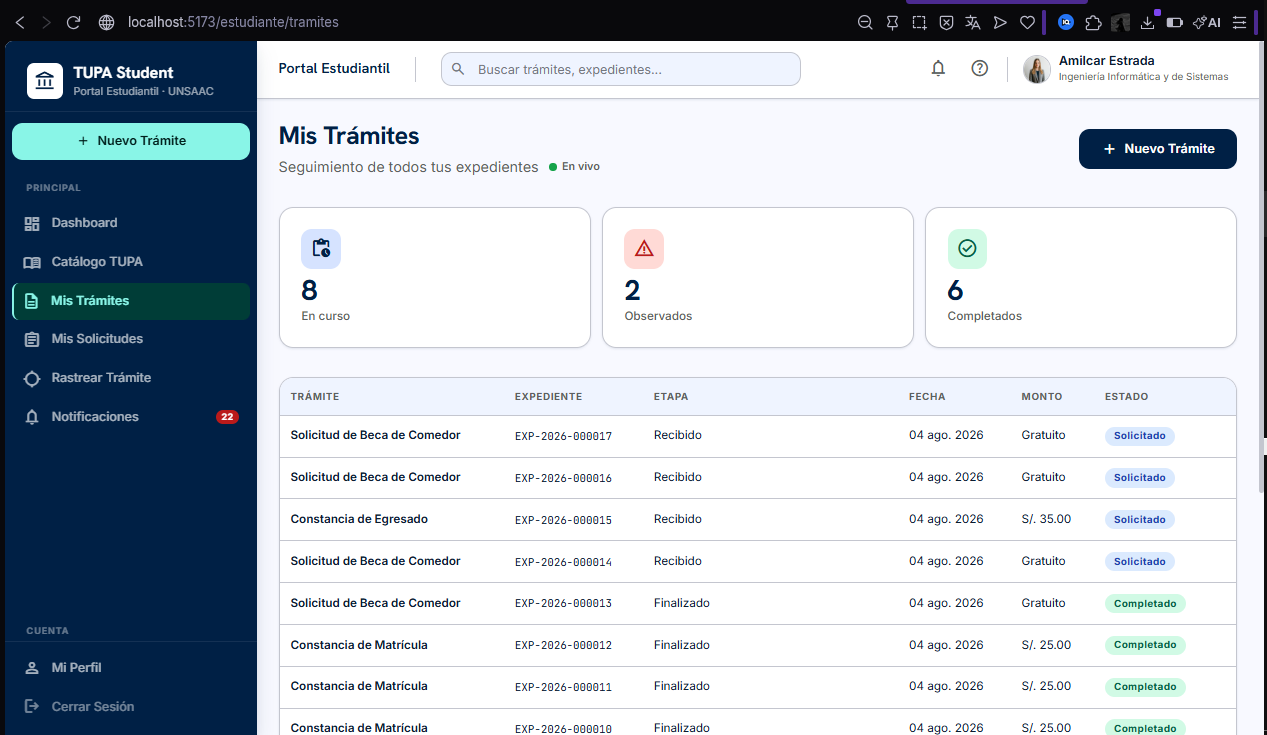
\includegraphics[width=0.95\linewidth]{images/estudiante-mis-tramites.png}%
}{Listado tabular de \emph{Mis Trámites} del estudiante, con etapa, monto y estado por expediente.}{fig:estudiante-mis-tramites}

\apafigure{%
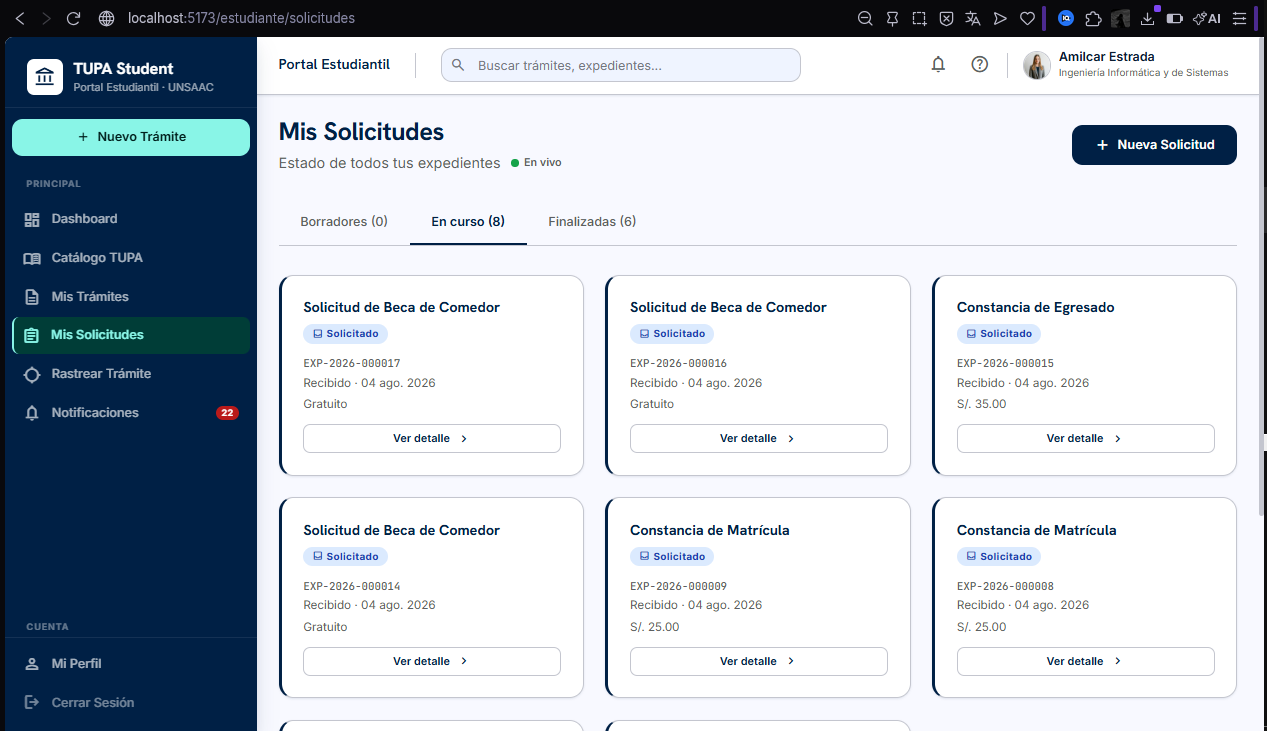
\includegraphics[width=0.95\linewidth]{images/estudiante-mis-solicitudes.png}%
}{Vista de \emph{Mis Solicitudes} organizada por pestañas de borradores, en curso y finalizadas.}{fig:estudiante-mis-solicitudes}

\apafigure{%
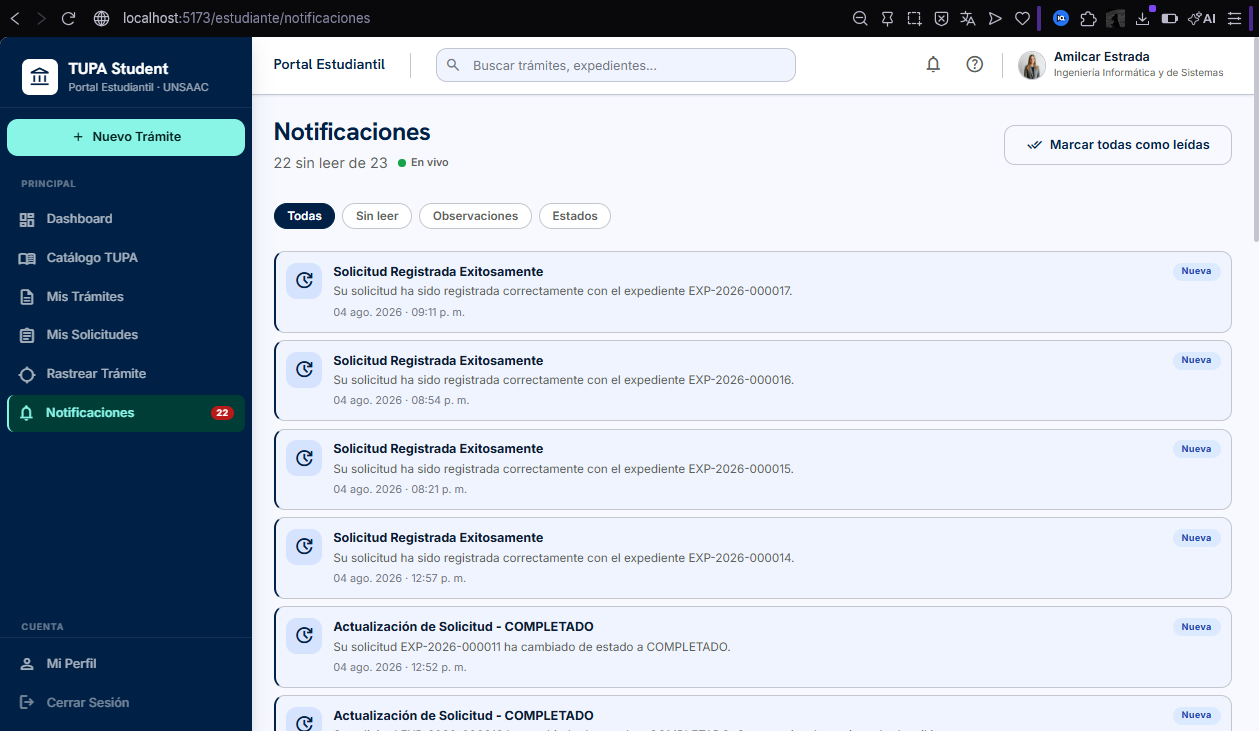
\includegraphics[width=0.95\linewidth]{images/estudiante-notificaciones.png}%
}{Centro de notificaciones del estudiante, con alertas de registro y cambios de estado de sus solicitudes.}{fig:estudiante-notificaciones}

\apafigure{%
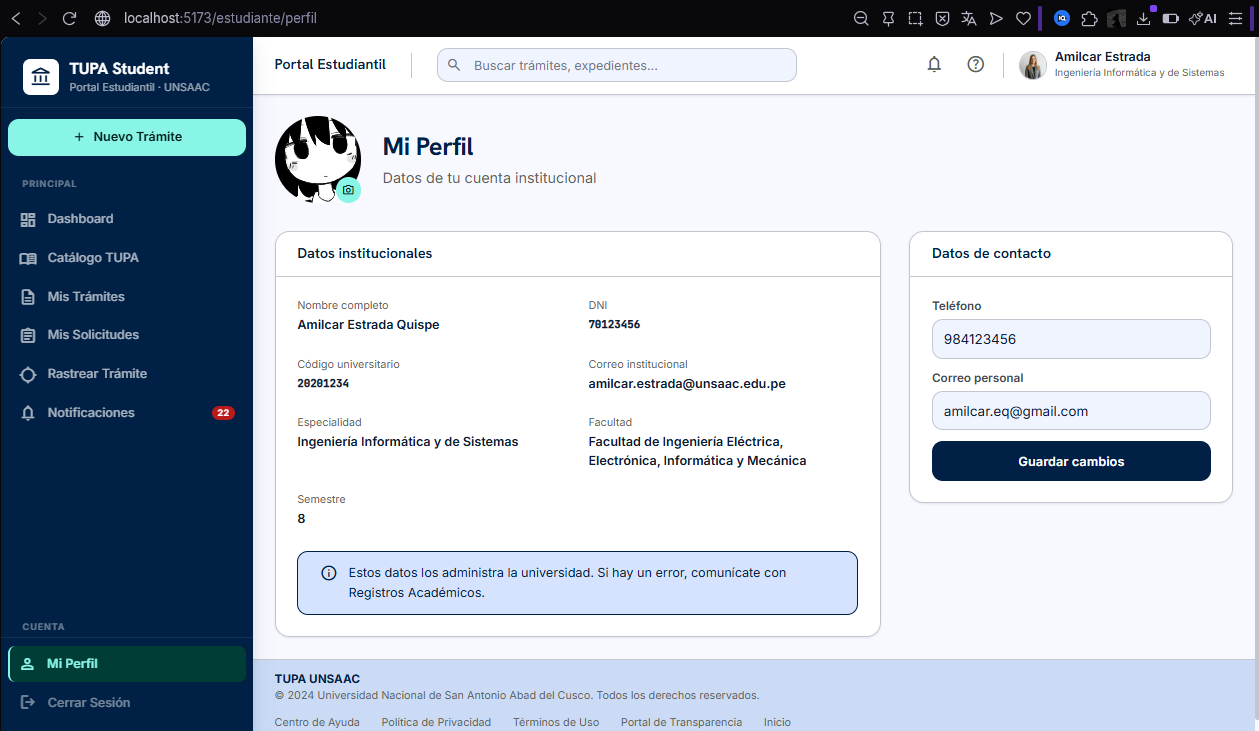
\includegraphics[width=0.95\linewidth]{images/estudiante-perfil.png}%
}{Pantalla \emph{Mi Perfil}, con datos institucionales de solo lectura, datos de contacto editables y carga de foto de perfil.}{fig:estudiante-perfil}

\subsubsection{Portal Administrativo}
El portal administrativo incluye el tablero de gestión con indicadores, la
cola de solicitudes pendientes, la validación documental, el detalle de
expediente donde se registra la decisión, la gestión del catálogo de
procedimientos, la administración de usuarios y el módulo de reportes. Estas
vistas se encuentran en \texttt{AdminDashboard.jsx},
\texttt{PendingQueue.jsx}, \texttt{DocumentValidation.jsx},
\texttt{RequestDetail.jsx}, \texttt{ProcedureManagement.jsx},
\texttt{UserManagement.jsx} y \texttt{Reports.jsx} dentro de
\texttt{frontend/src/pages/admin/}.

\apafigure{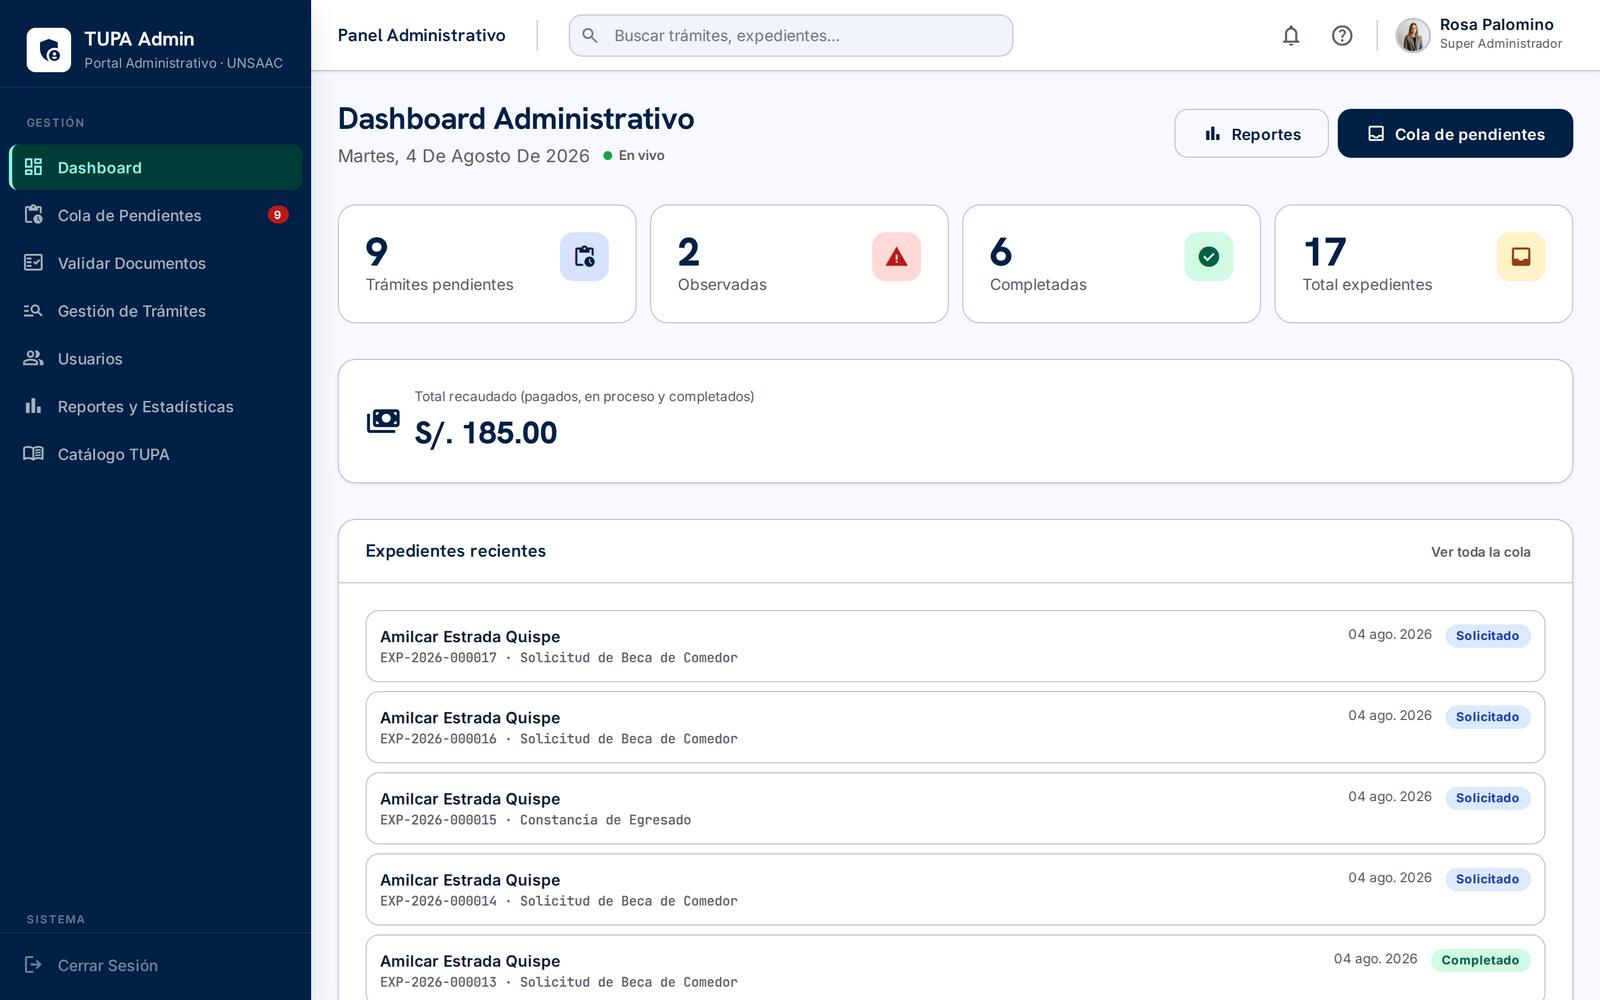
\includegraphics[width=0.95\textwidth]{images/capt-adm-dashboard.png}}%
{Tablero administrativo con indicadores agregados y expedientes recientes (ruta \texttt{/admin}).}{fig:adm-dashboard}

\apafigure{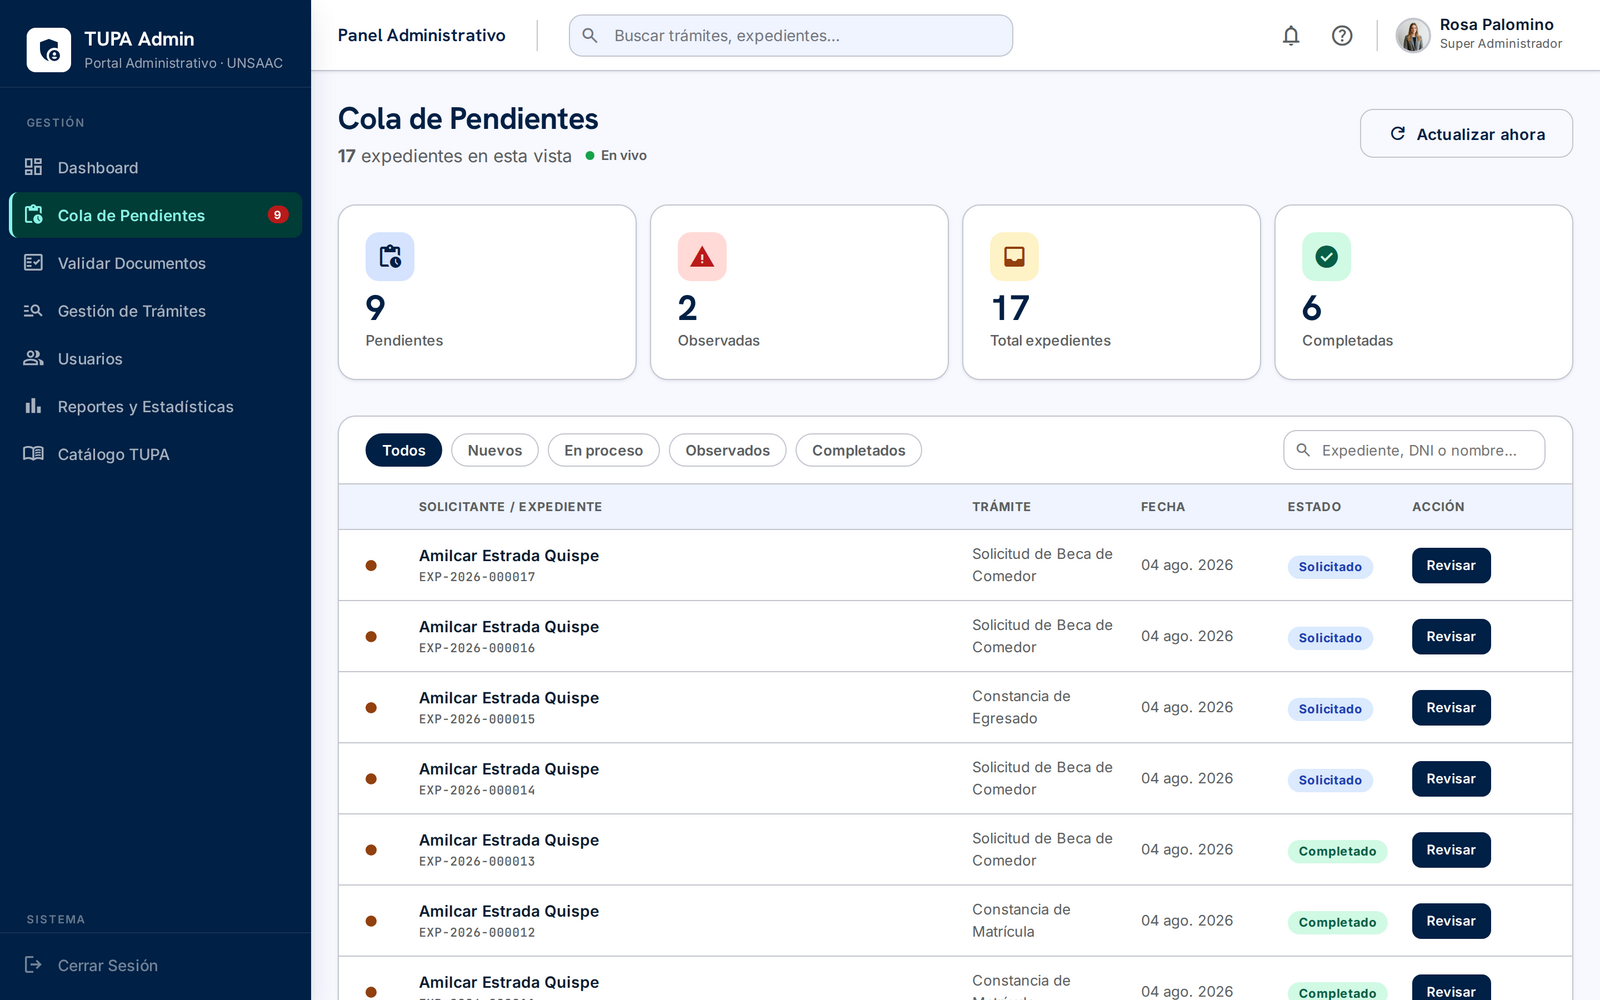
\includegraphics[width=0.95\textwidth]{images/capt-adm-cola.png}}%
{Cola de solicitudes pendientes de atención (ruta \texttt{/admin/cola}).}{fig:adm-cola}

\apafigure{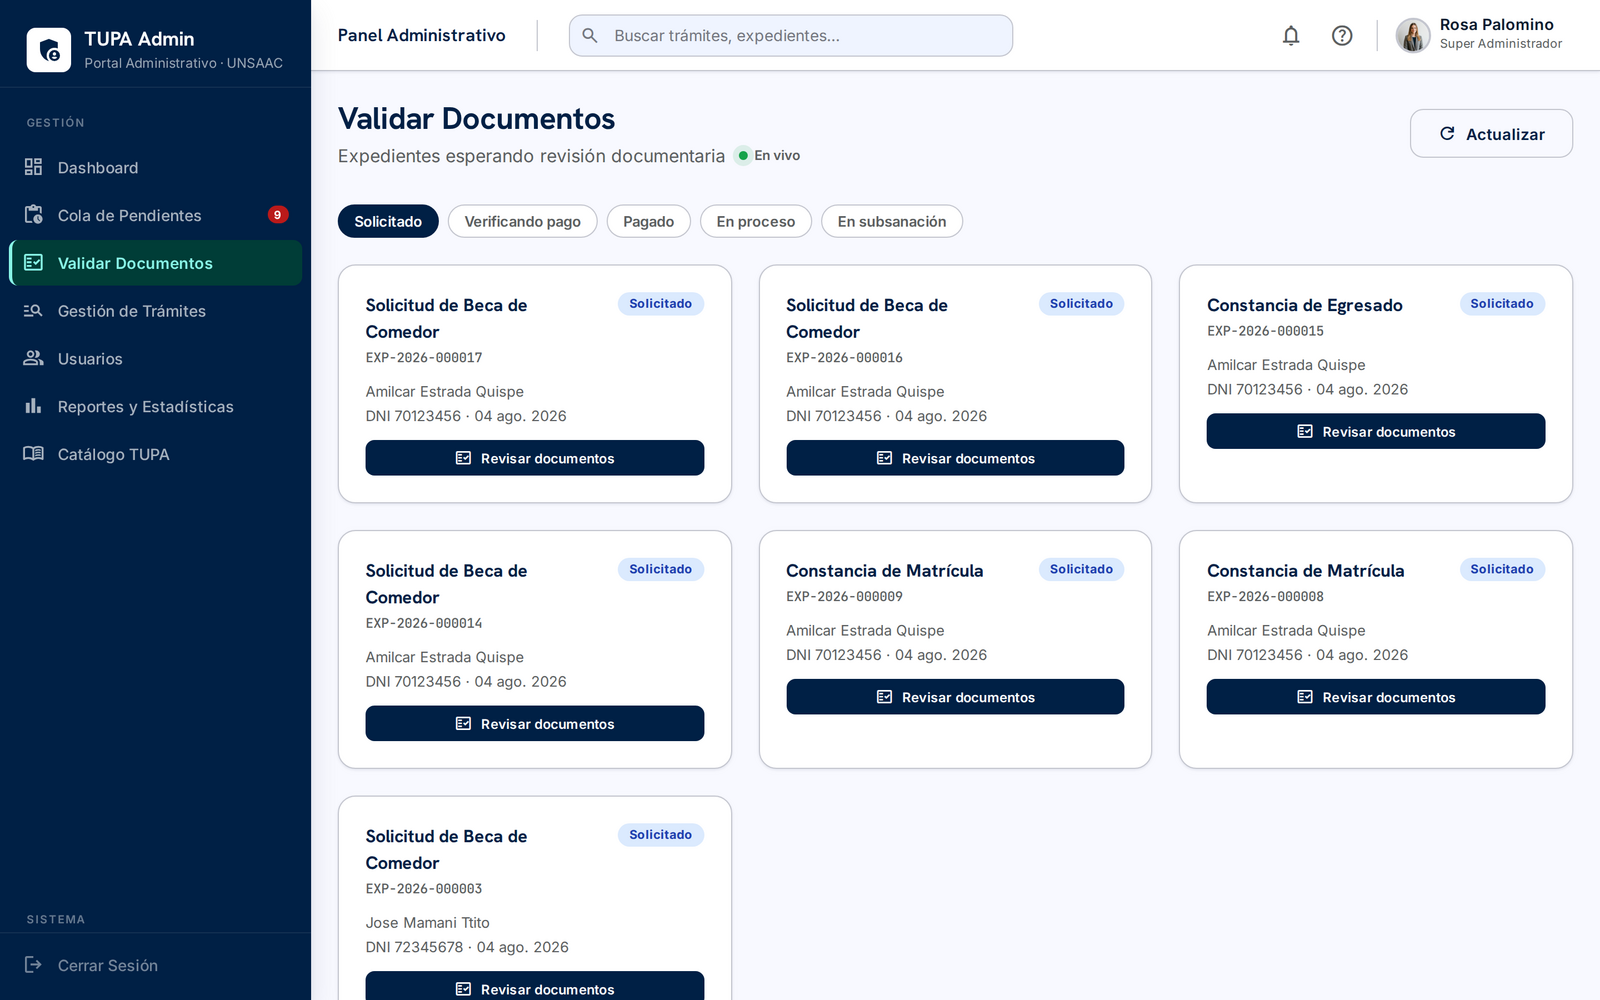
\includegraphics[width=0.95\textwidth]{images/capt-adm-validacion.png}}%
{Validación documentaria de los archivos cargados (ruta \texttt{/admin/validacion}).}{fig:adm-validacion}

\apafigure{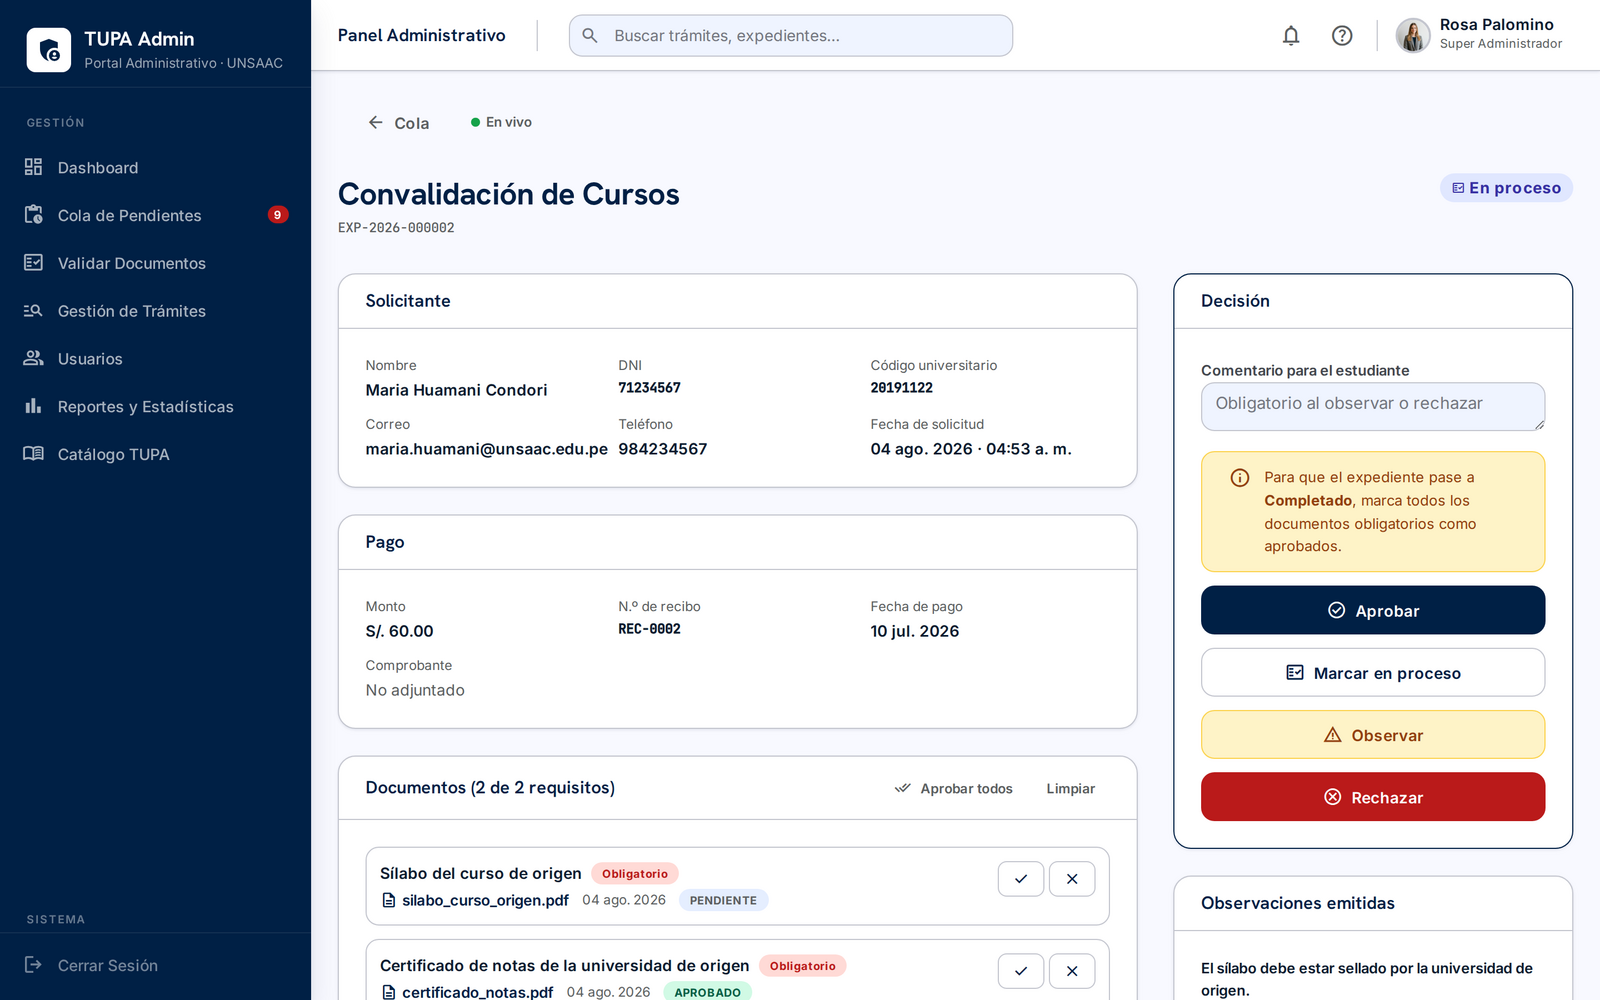
\includegraphics[width=0.95\textwidth]{images/capt-adm-solicitud-detalle.png}}%
{Detalle de expediente y registro de la decisión administrativa (ruta \texttt{/admin/solicitudes/:id}).}{fig:adm-solicitud-detalle}

\apafigure{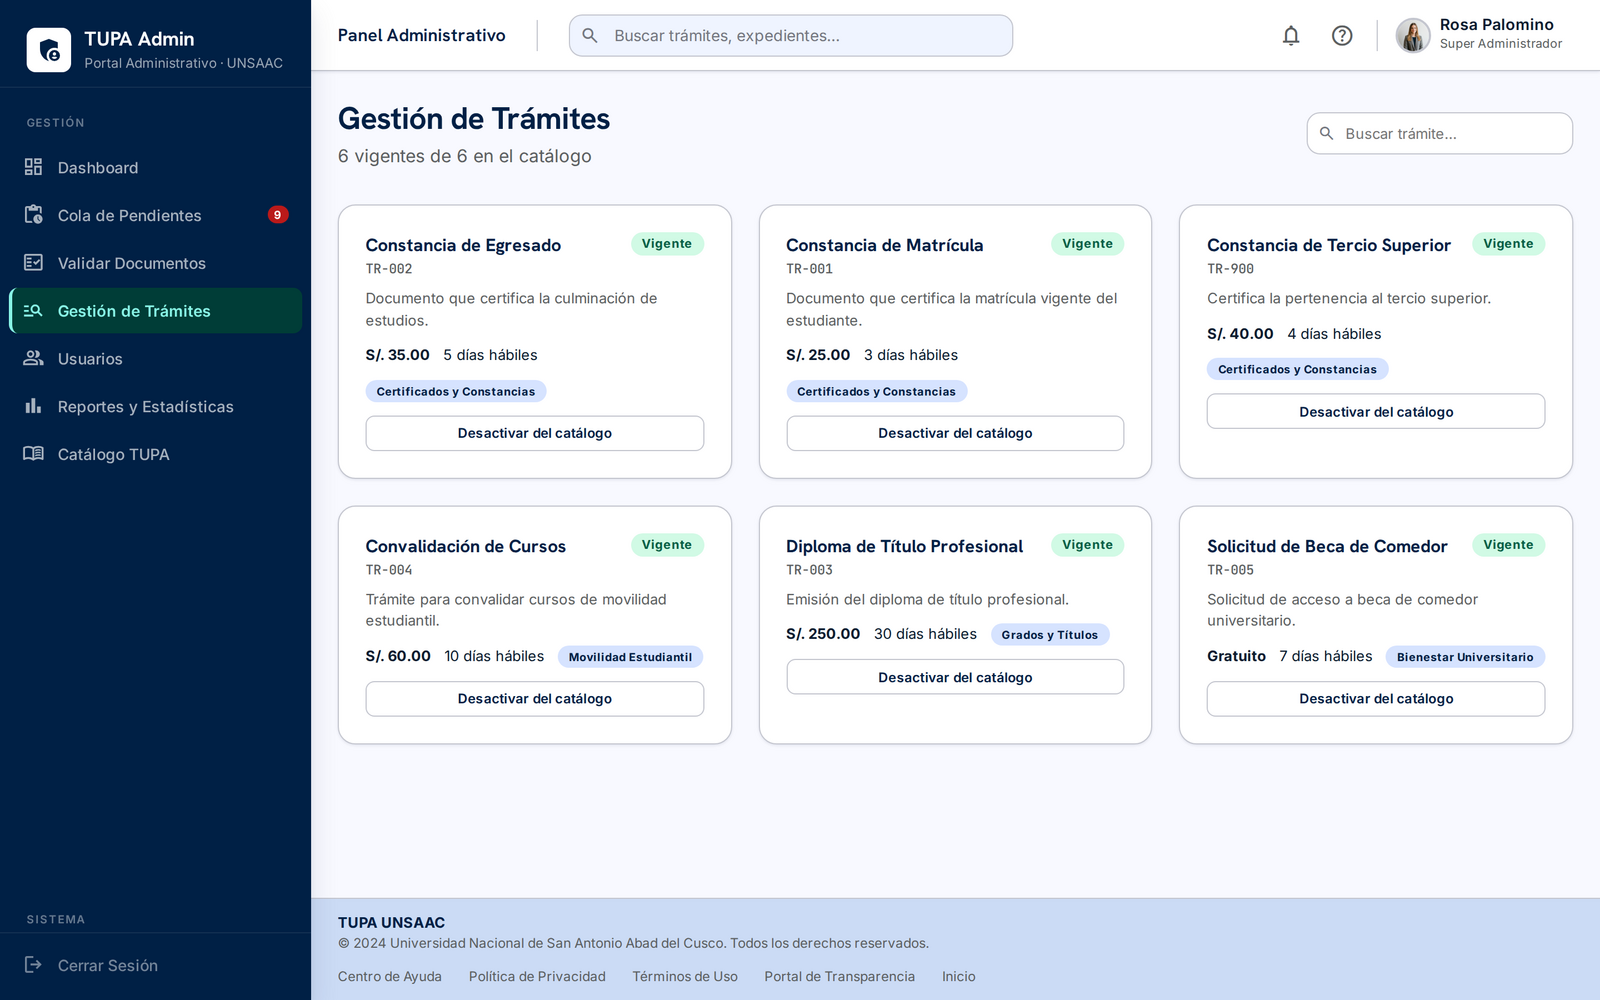
\includegraphics[width=0.95\textwidth]{images/capt-adm-procedimientos.png}}%
{Gestión del catálogo de trámites del TUPA (ruta \texttt{/admin/procedimientos}).}{fig:adm-procedimientos}

\apafigure{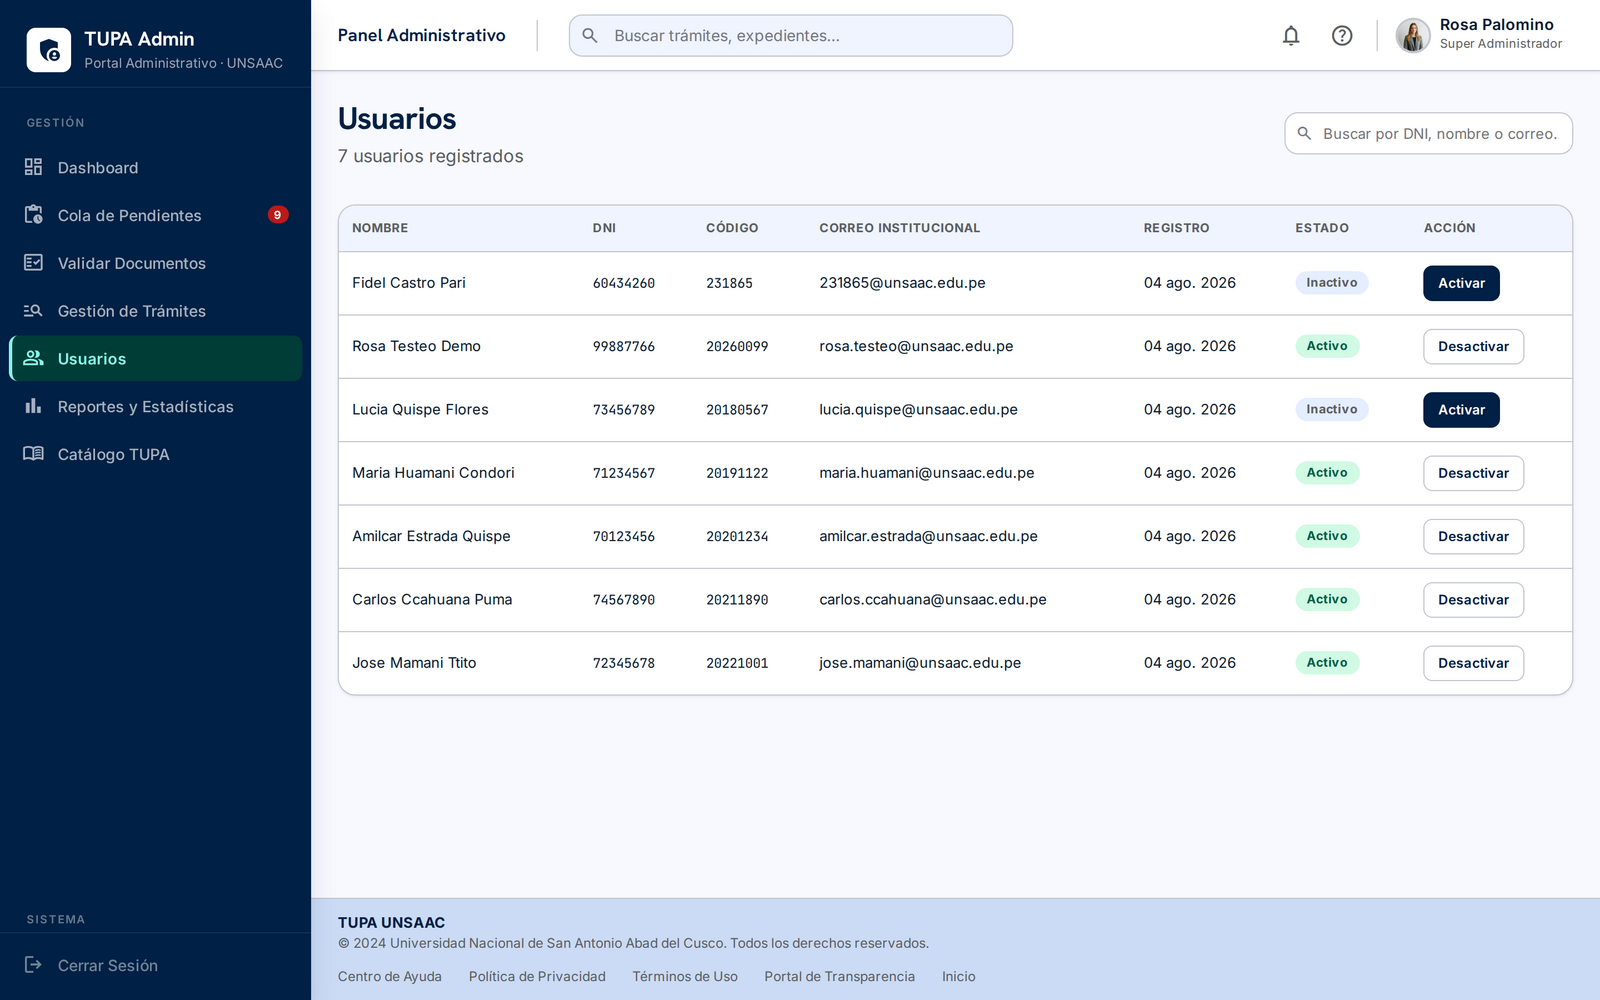
\includegraphics[width=0.95\textwidth]{images/capt-adm-usuarios.png}}%
{Administración de usuarios registrados (ruta \texttt{/admin/usuarios}).}{fig:adm-usuarios}

\apafigure{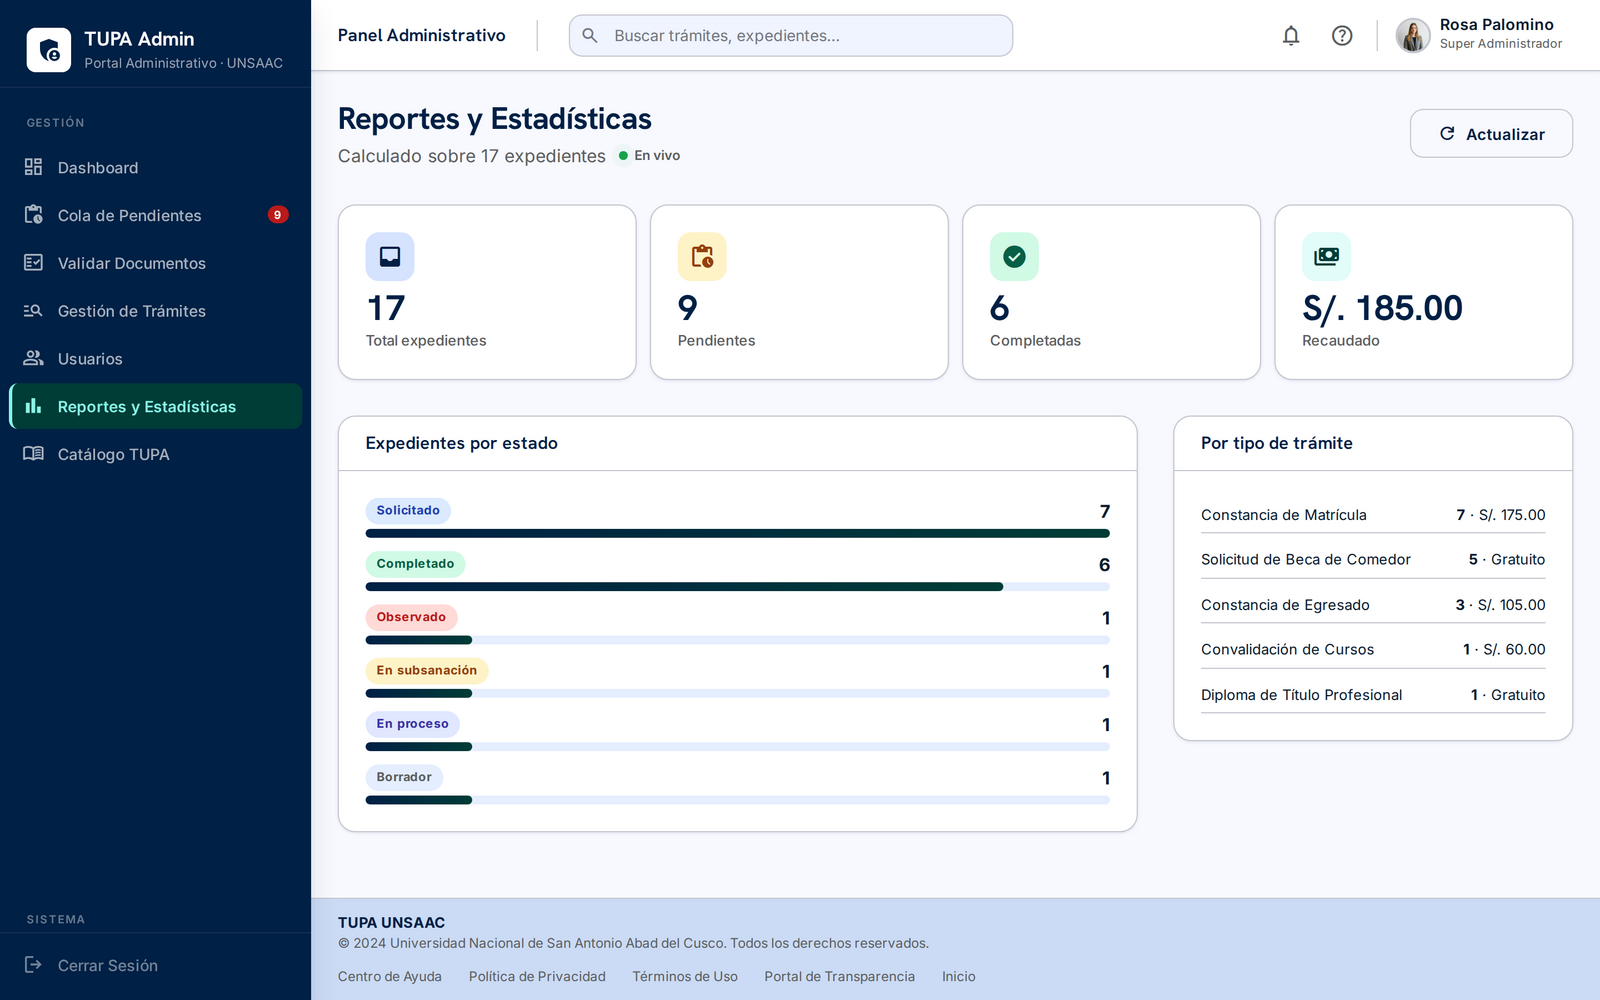
\includegraphics[width=0.95\textwidth]{images/capt-adm-reportes.png}}%
{Reportes y estadísticas del sistema (ruta \texttt{/admin/reportes}).}{fig:adm-reportes}

\subsubsection{Componente Pendiente}
La ruta \texttt{/seguimiento/detalle}, servida por
\texttt{ProcedureTimeline.jsx}, conserva datos de ejemplo escritos
directamente en el componente y no consume la API. Se documenta aquí como
elemento pendiente de integración: la funcionalidad equivalente sí está
resuelta y conectada en el detalle de expediente del estudiante
(Figura~\ref{fig:est-solicitud-detalle}) y en el resultado de la consulta
pública (Figura~\ref{fig:seguimiento-resultados}).

\apafigure{%
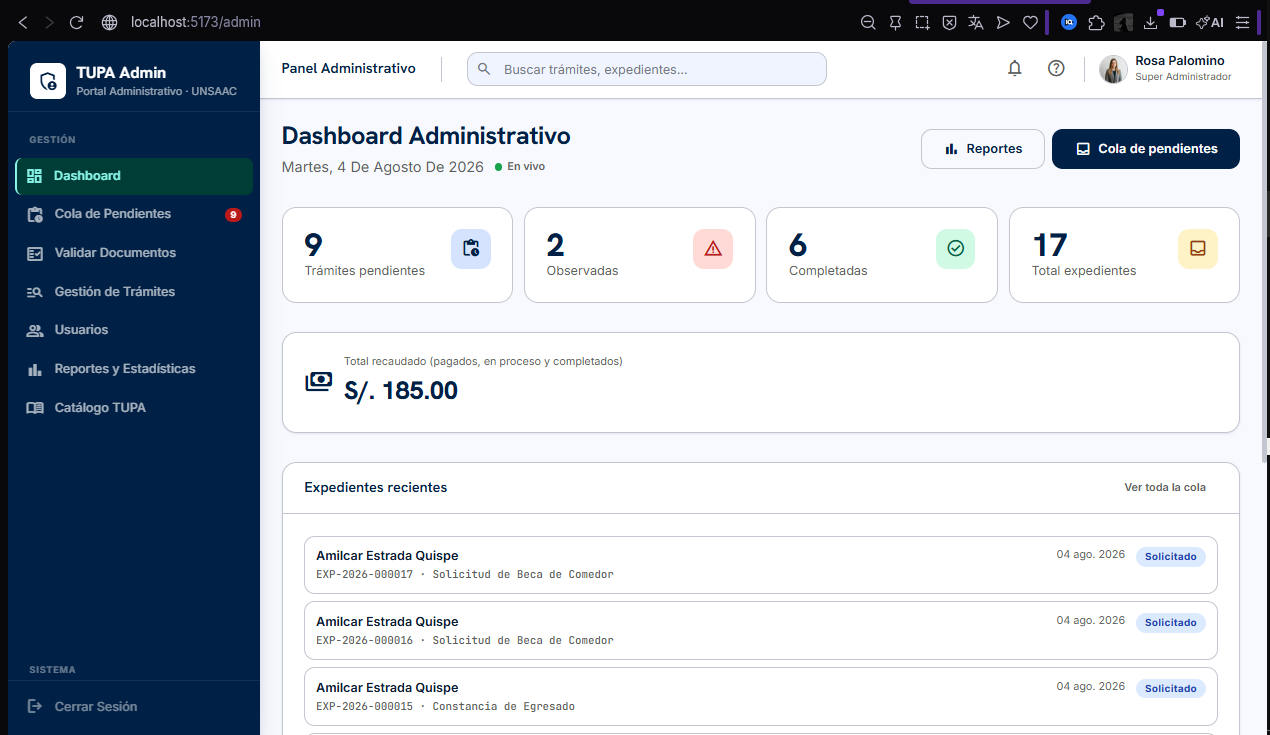
\includegraphics[width=0.95\linewidth]{images/admin-dashboard.png}%
}{Dashboard administrativo, con indicadores de trámites pendientes, observados, completados y monto total recaudado.}{fig:admin-dashboard}

\apafigure{%
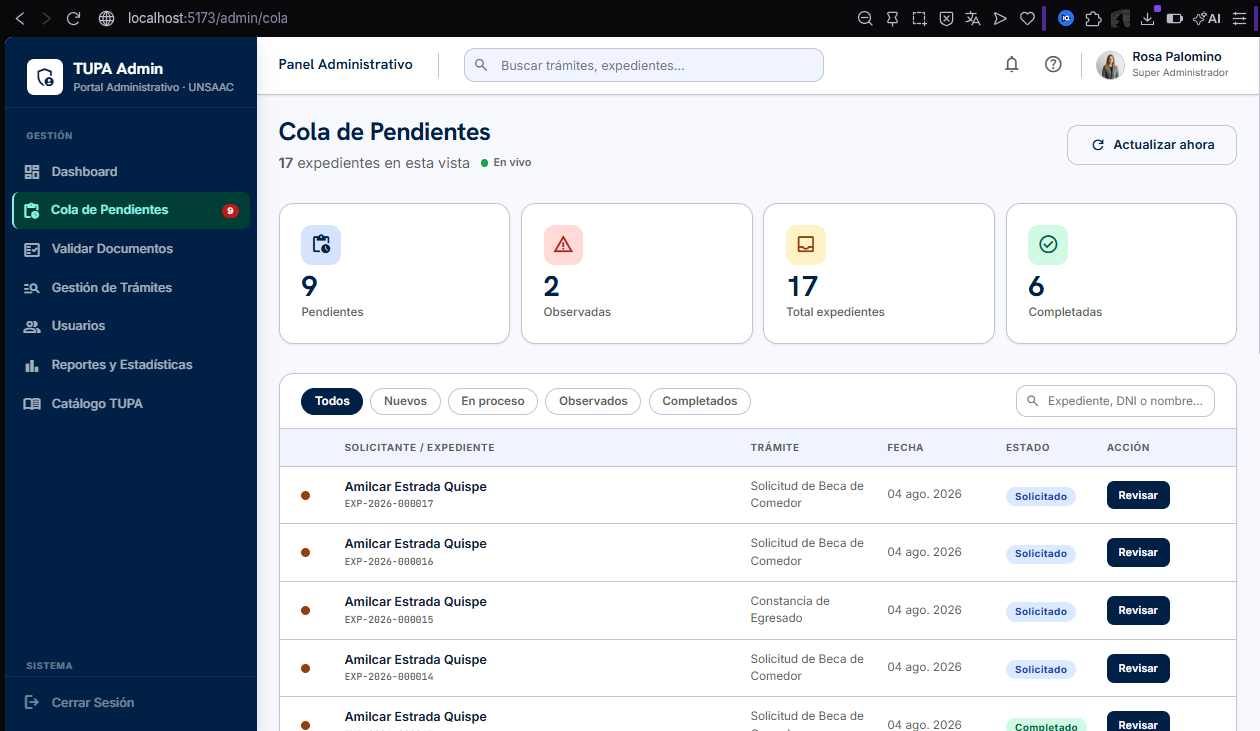
\includegraphics[width=0.95\linewidth]{images/admin-cola-pendientes.png}%
}{Cola de pendientes administrativa, con filtros por estado y acceso directo a la revisión de cada expediente.}{fig:admin-cola-pendientes}

\apafigure{%
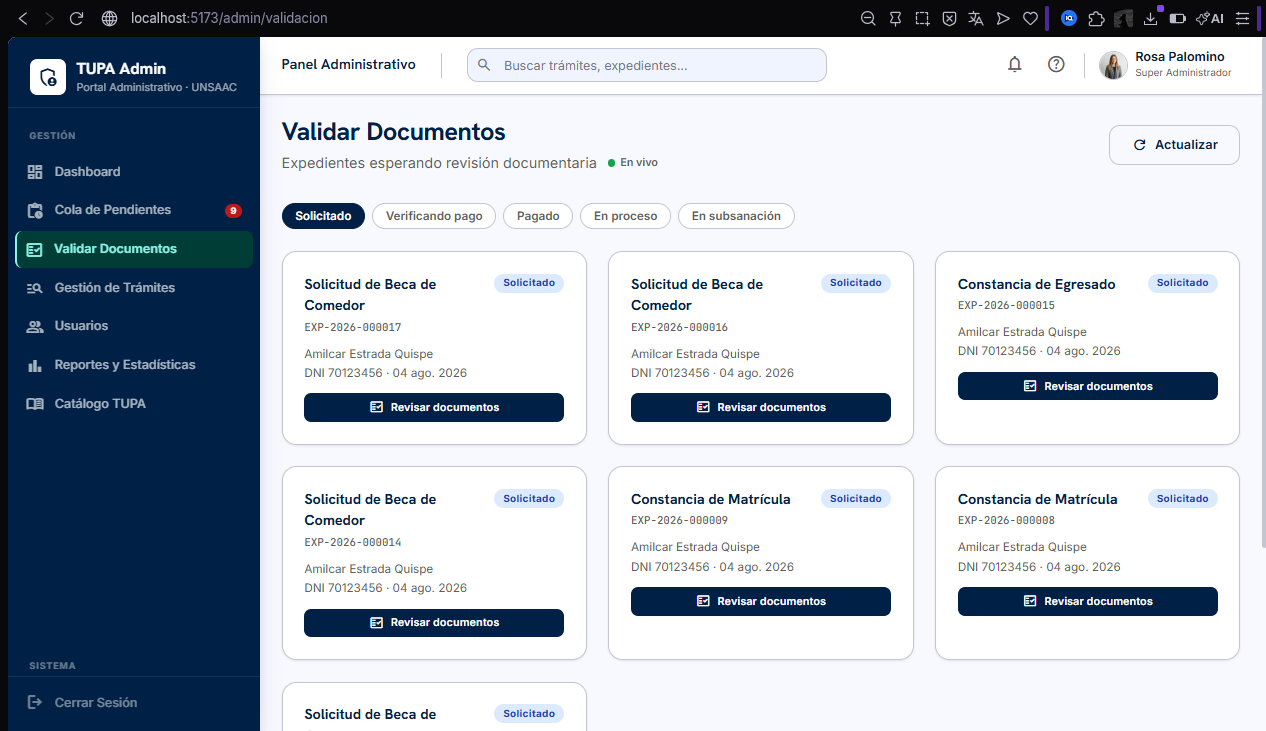
\includegraphics[width=0.95\linewidth]{images/admin-validar-documentos.png}%
}{Vista de validación documental, con los expedientes agrupados por etapa a la espera de revisión.}{fig:admin-validar-documentos}

\apafigure{%
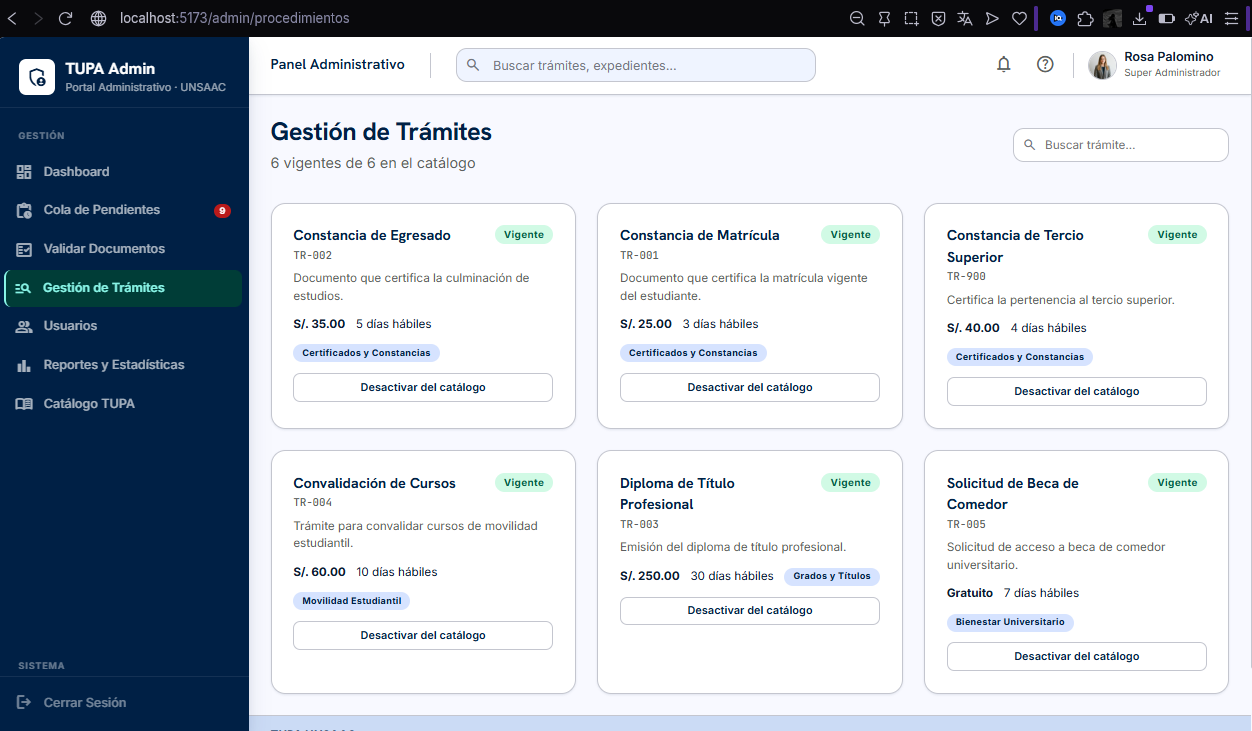
\includegraphics[width=0.95\linewidth]{images/admin-gestion-tramites.png}%
}{Gestión del catálogo de trámites, con activación/desactivación de procedimientos vigentes.}{fig:admin-gestion-tramites}

\apafigure{%
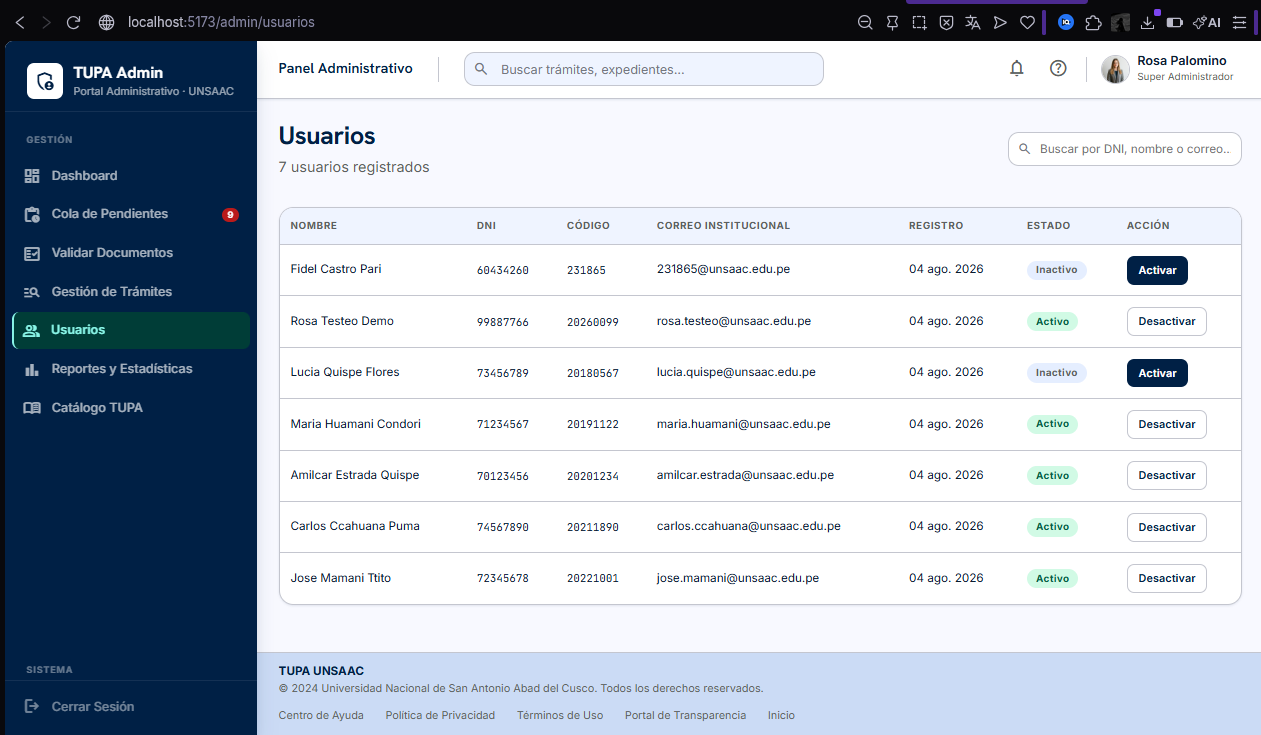
\includegraphics[width=0.95\linewidth]{images/admin-usuarios.png}%
}{Administración de usuarios registrados, con activación y desactivación de cuentas.}{fig:admin-usuarios}

\apafigure{%
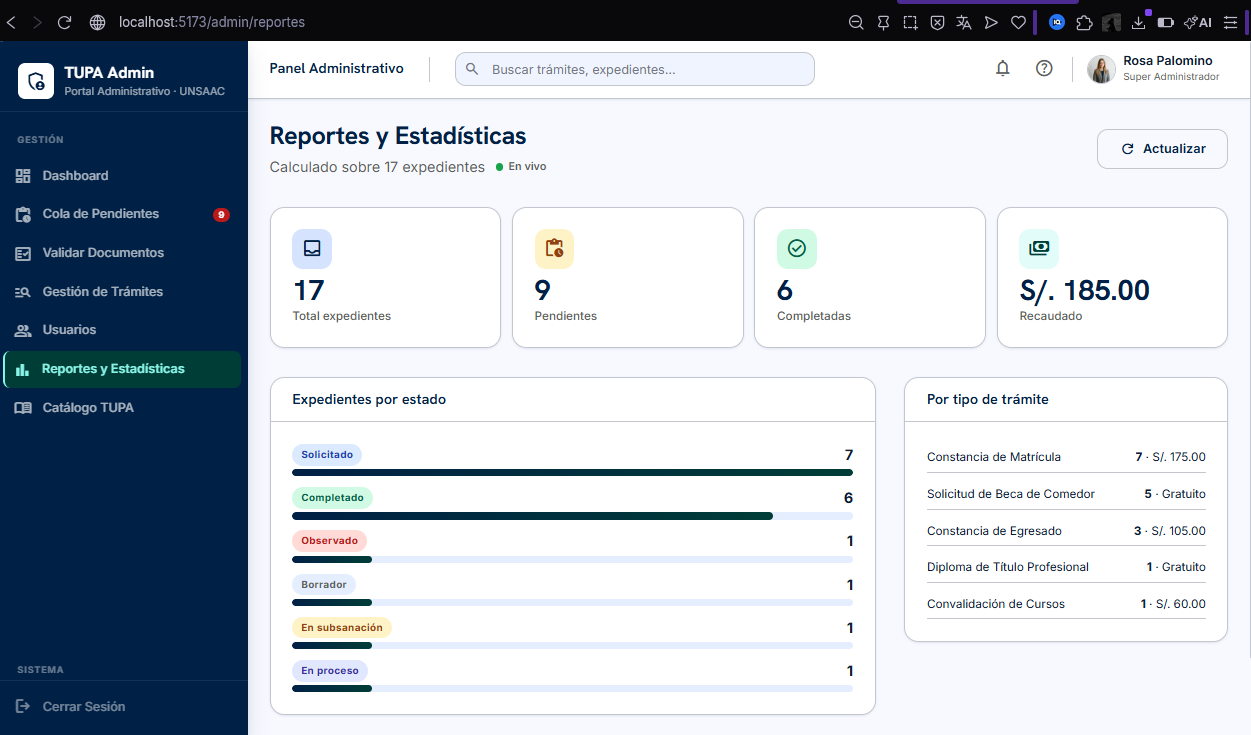
\includegraphics[width=0.95\linewidth]{images/admin-reportes.png}%
}{Panel de reportes y estadísticas, con expedientes por estado y por tipo de trámite.}{fig:admin-reportes}

\subsection{Seguridad}
El sistema implementa los siguientes mecanismos de seguridad a nivel de API:
\begin{itemize}
    \item \textbf{Autenticación:} el middleware \texttt{authenticateToken}
    intercepta las rutas protegidas, valida el token JWT recibido en la
    cabecera \texttt{Authorization: Bearer <token>} y adjunta la identidad
    del usuario a la petición.
    \item \textbf{Autorización por rol:} el middleware
    \texttt{requireRole('ADMIN')} restringe el acceso a las rutas bajo
    \texttt{/api/admin} a los tokens cuyo campo \texttt{role} sea
    \texttt{ADMIN}, devolviendo \texttt{403} en caso contrario.
    \item \textbf{Verificación de pertenencia:} además del rol, los servicios
    de solicitudes y documentos comprueban que el recurso pertenezca al
    usuario que lo pide, distinguiendo \texttt{404} (no existe) de
    \texttt{403} (existe pero es de otro usuario).
    \item \textbf{Cifrado de contraseñas:} las contraseñas se almacenan
    como \emph{hash} \texttt{bcrypt} con 10 rondas de sal, nunca en texto
    plano. La política exige entre 8 y 64 caracteres con minúscula,
    mayúscula, dígito y símbolo.
    \item \textbf{Sesiones de doble token:} se emiten un token de acceso de
    15 minutos y uno de renovación de 7 días, firmados con secretos
    distintos. El token de renovación se persiste en la tabla
    \texttt{refresh\_token} y rota en cada uso: el anterior queda revocado.
    Cambiar la contraseña elimina todas las sesiones abiertas del usuario.
    \item \textbf{Limitación de intentos:} \texttt{rateLimit.middleware}
    restringe por IP los endpoints de inicio de sesión, registro y
    recuperación de contraseña, respondiendo \texttt{429} con cabecera
    \texttt{Retry-After} al superar el umbral. Los códigos de recuperación
    admiten un máximo de cinco intentos antes de invalidarse.
    \item \textbf{No divulgación de cuentas:} el inicio de sesión devuelve el
    mismo mensaje ante usuario inexistente y contraseña incorrecta, y la
    verificación de la cuenta activa se realiza después de comprobar la
    contraseña. Los endpoints de recuperación y reenvío responden siempre con
    un mensaje genérico.
    \item \textbf{Validación de archivos:} \texttt{multer} acepta únicamente
    PDF, JPG, JPEG y PNG, con un límite de 5~MB por archivo. Los archivos se
    guardan en columnas \texttt{BYTEA} de PostgreSQL y no en el sistema de
    archivos, dado que el backend se despliega sobre una plataforma
    \emph{serverless} de disco efímero.
    \item \textbf{Prevención de inyección SQL:} todas las consultas a la
    base de datos se ejecutan mediante sentencias parametrizadas.
    \item \textbf{Manejo centralizado de errores:} el middleware de errores
    traduce los códigos de restricción de PostgreSQL a respuestas
    \texttt{400}/\texttt{409} y sustituye por un mensaje genérico cualquier
    error \texttt{500}, evitando filtrar detalles internos al cliente.
\end{itemize}

\paragraph{Limitación conocida.} La política de CORS se configura desde la
variable \texttt{CLIENT\_ORIGIN} como una lista de orígenes separados por
comas; cuando dicha variable no está definida, el backend acepta peticiones
desde cualquier origen. Esta decisión se tomó para permitir la demostración
en red local desde una segunda máquina, pero en un despliegue de producción
la variable debe fijarse explícitamente.

\subsection{Despliegue}
El proyecto contempla dos modos de ejecución. Para desarrollo y demostración,
el backend se ejecuta con Node.js sobre el puerto \texttt{3000} y el frontend
se sirve con Vite sobre el puerto \texttt{5173}; el cliente resuelve la URL de
la API tomando el mismo nombre de host desde el que se sirve la página y el
puerto 3000, de modo que la demostración funciona en red local sin
reconfiguración. Para el despliegue, el repositorio incluye un archivo
\texttt{vercel.json} y el backend está adaptado a un entorno
\emph{serverless}: por eso ningún archivo se persiste en disco y tanto los
documentos como los avatares se almacenan en PostgreSQL. La base de datos
utilizada durante el desarrollo está alojada en un servicio gestionado
externo. Las variables de entorno necesarias se registran en el archivo
\texttt{.env} del backend e incluyen la cadena de conexión a PostgreSQL, los
secretos de firma JWT, el puerto HTTP y las credenciales del servidor de
correo saliente.

\subsection{Pruebas}
La verificación del sistema se realizó con pruebas automatizadas mediante Jest
y Supertest. La suite se organiza por módulo, cubre los siete módulos del
backend y consta de \textbf{6 suites} con \textbf{169 pruebas}, todas en
verde en la última ejecución. Se emplean dos estrategias complementarias:

\begin{itemize}
    \item \textbf{Pruebas de integración HTTP:} levantan la aplicación
    Express con \texttt{supertest} y sustituyen la capa de servicios por
    dobles de prueba (\texttt{jest.mock}). Ejercitan el enrutado, los
    middlewares de autenticación y autorización, la validación de archivos y
    la forma de las respuestas sin requerir una base de datos activa, lo que
    las hace reproducibles en cualquier máquina y en integración continua.
    \item \textbf{Pruebas unitarias sin dobles:} ejecutan el código real de
    las utilidades, que son funciones puras o dependen únicamente de un
    cliente de base de datos simulable con un objeto. Con ello se verifica
    lógica de negocio efectiva y no sólo el cableado entre capas.
\end{itemize}

\apatable{%
\footnotesize
\begin{tabular}{@{}>{\raggedright\arraybackslash}p{5.5cm}p{1.1cm}>{\raggedright\arraybackslash}p{7.9cm}@{}}
\toprule
\textbf{Archivo} & \textbf{Casos} & \textbf{Cobertura} \\
\midrule
\texttt{auth.test.js} & 22 & Health check, inicio de sesión (incluidos 401 y 403), registro, activación e idempotencia del enlace, renovación y cierre de sesión, recuperación de contraseña y límite de intentos. \\
\texttt{users-procedures.test.js} & 42 & Perfil y campos no editables, cambio de contraseña, avatares, catálogo y filtros, y el flujo completo de solicitudes con sus reglas de pertenencia. \\
\texttt{middleware.test.js} & 33 & Autenticación sin token, con firma inválida o expirada; guardián de rol sobre las ocho rutas administrativas; ruta inexistente; traducción de errores de PostgreSQL; validación de tipo y tamaño de archivo. \\
\texttt{utils.test.js} & 32 & Código real de \texttt{validate}, \texttt{generateExpediente}, \texttt{jwt.util} y \texttt{asyncHandler}. \\
\texttt{admin.test.js} & 21 & Estadísticas, cola de solicitudes, decisión administrativa con sus validaciones y conflictos, gestión de trámites y usuarios. \\
\texttt{documents-notifications.test.js} & 19 & Visualización y eliminación de documentos con control de pertenencia, listado y marcado de notificaciones. \\
\bottomrule
\end{tabular}%
}{Organización de la suite de pruebas automatizadas del backend.}{tab:pruebas}

Además de los casos de camino feliz, la suite verifica de forma explícita los
caminos de error: peticiones sin token (\texttt{401}), token con firma
inválida o expirado (\texttt{403}), rol insuficiente sobre cada una de las
ocho rutas de \texttt{/api/admin} (\texttt{403}), identificadores mal formados
(\texttt{400}), recursos inexistentes (\texttt{404}), conflictos de estado al
reenviar una solicitud ya enviada o al decidir sobre un expediente cerrado
(\texttt{409}) y exceso de intentos en los endpoints de autenticación
(\texttt{429}). Se comprueba también que un error inesperado responda
\texttt{500} con un mensaje genérico, sin filtrar detalles internos de la
base de datos. La suite se ejecuta con \texttt{npm test} desde el directorio
\texttt{backend/}.

\apafigure{%
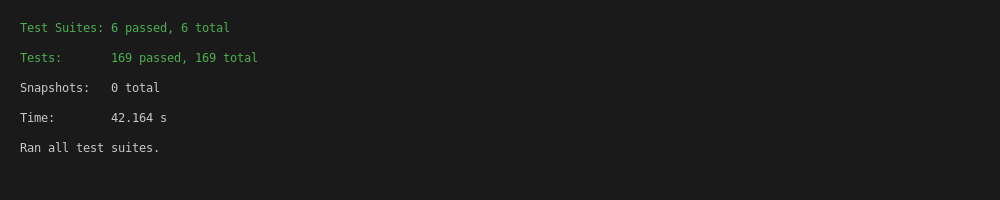
\includegraphics[width=0.95\textwidth]{images/capt-test-output.png}%
}{Ejecución completa de la suite de 169 pruebas automatizadas.}{fig:test-output}

\subsection{Historial de Commits}

El desarrollo del proyecto ha transitado por diez hitos principales documentados
en el control de versiones. Estos reflejan la construcción incremental de los
componentes de infraestructura (almacenamiento, autenticación, integración de
servicios), la verificación de funcionalidad mediante pruebas, y la preparación
para despliegue.

\apafigure{%
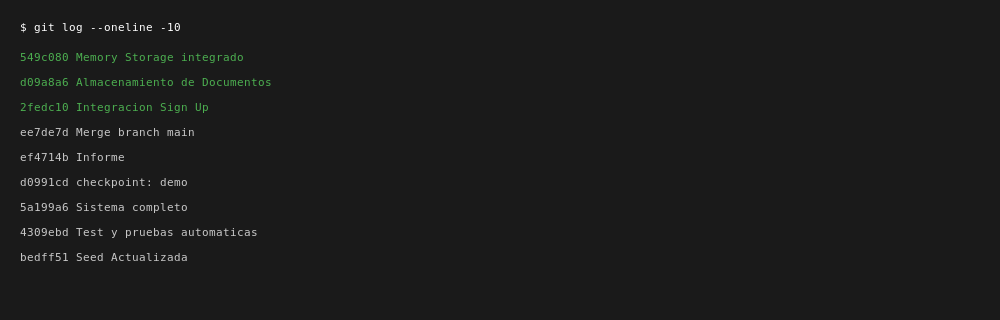
\includegraphics[width=0.95\textwidth]{images/capt-git-log.png}%
}{Historial de commits del repositorio, mostrando los diez últimos puntos de control.}{fig:git-log}
